\documentclass[11pt]{article}
\usepackage[utf8]{inputenc}
\usepackage[dvips]{graphicx}
\usepackage{fancybox}
\usepackage{verbatim}
\usepackage{multirow,array}
\usepackage{latexsym}
\usepackage{alltt}
\usepackage{hyperref}
\usepackage{textcomp}
\usepackage{color}
\usepackage{amsmath}
\usepackage{amsfonts}
\usepackage{tikz}
\usepackage{float}
\usepackage[hmargin=3cm,vmargin=5.0cm]{geometry}
%\topmargin=0cm
\topmargin=-2cm
\addtolength{\textheight}{6.5cm}
\addtolength{\textwidth}{2.0cm}
%\setlength{\leftmargin}{-5cm}
\setlength{\oddsidemargin}{0.0cm}
\setlength{\evensidemargin}{0.0cm}


\begin{document}

\section*{Student Information } 
%Write your full name and id number between the colon and newline
%Put one empty space character after colon and before newline
Full Name : Onat ÖZDEMİR \\
Id Number : 2310399 \\

% Write your answers below the section tags

\section*{Answer 1}
\subsection*{a)}
\begin{figure}[H]
	\centering
	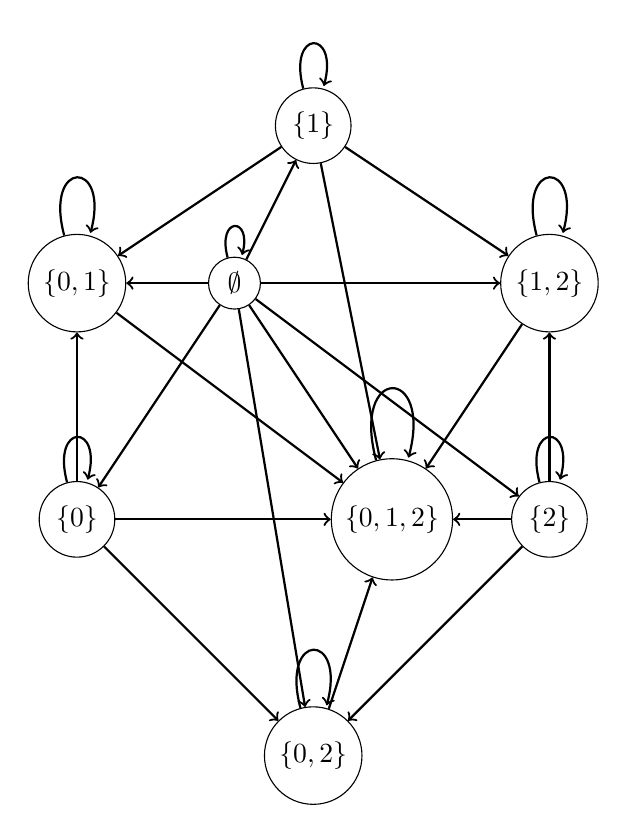
\begin{tikzpicture}
	
\node[shape=circle,draw=black] (a) at (3, 0)     {\textbf{$\{0,2\}$}};
\node[shape=circle,draw=black] (b) at (4, 3)     {\textbf{$\{0,1,2\}$}};
\node[shape=circle,draw=black] (c) at (0, 3)     {\textbf{$\{0\}$}};
\node[shape=circle,draw=black] (d) at (6, 3)     {\textbf{$\{2\}$}};
\node[shape=circle,draw=black] (e) at (0, 6)     {\textbf{$\{0,1\}$}};
\node[shape=circle,draw=black] (f) at (2, 6)     {\textbf{$\emptyset$}};
\node[shape=circle,draw=black] (g) at (6, 6)     {\textbf{$\{1,2\}$}};
\node[shape=circle,draw=black] (h) at (3, 8)     {\textbf{$\{1\}$}};
	

	\path[->, thick] (f) edge (a);
	\path[->, thick] (f) edge (b);
	\path[->, thick] (f) edge (c);
	\path[->, thick] (f) edge (d);
	\path[->, thick] (f) edge (e);
	\path[->, thick] (f) edge [loop above] (f);
	\path[->, thick] (f) edge (g);
	\path[->, thick] (f) edge (h);
	\path[->, thick] (c) edge (a);
	\path[->, thick] (c) edge (e);
	\path[->, thick] (c) edge (b);
	\path[->, thick] (c) edge [loop above] (c);
	\path[->, thick] (h) edge (b);
	\path[->, thick] (h) edge (e);
	\path[->, thick] (h) edge (g);
	\path[->, thick] (h) edge [loop above] (h);
	\path[->, thick] (d) edge (b);
	\path[->, thick] (d) edge (a);
	\path[->, thick] (d) edge (g);
	\path[->, thick] (d) edge [loop above] (d);
	\path[->, thick] (e) edge (b);
	\path[->, thick] (e) edge [loop above] (e);
	\path[->, thick] (g) edge (b);
	\path[->, thick] (g) edge [loop above] (g);
    \path[->, thick] (a) edge (b);
    \path[->, thick] (a) edge [loop above] (a);
    \path[->, thick] (b) edge [loop above] (b);
    
	
	
	\end{tikzpicture} 
\end{figure}
\subsection*{b)}
In order to prove (S,R) is a poset, firstly we must prove that R is a reflexive, antisymmetric and transitive relation on S. \\
\textbf{Proof of R is Reflexive:}
In order to prove R is a reflexive relation, we have to prove that $\forall x\in S \ (xRx)$. According to the theorem placed in Rosen's Discrete Mathematics and Its Applications book, page 120, THEOREM1 for every set A, $A \subseteq A$ satisfies. Then, according to the definition of S, since each $x\in S$ is a set,
\begin{equation*}
\begin{split}
\forall x\in S \ (x\subseteq x)
\end{split}
\end{equation*}
Then,
\begin{equation*}
\begin{split}
\forall x\in S \ (xRx)
\end{split}
\end{equation*}
Thus, by the definition, we have proved that R is a reflexive relation on S.\\
\textbf{Proof of R is Antisymmetric:}
In order to prove R is an antisymmetric relation, we have to prove that $\forall x,y\in S \ ((xRy \land yRx)\rightarrow(x=y))$. Let $x$ and $y$ be arbitrarily chosen elements of S, if $x \subseteq y$ and $y \subseteq x$ then by the Axiom of Extensionality we can conclude that $x = y$. Since we choose $x$ and $y$ arbitrarily then, we can conclude that $\forall x,y\in S \ ((x \subseteq y \land y\subseteq x)\rightarrow(x=y))$. Hence, we have proved that $\forall x,y\in S \ ((xRy \land yRx)\rightarrow(x=y))$. Thus, by the definition, R is an antisymmetric relation. \\
\textbf{Proof of R is Transitive:} In order to prove R is a transitive relation, we need to prove that $\forall x,y,z\in S \ ((xRy\land yRz) \rightarrow xRz)$. Let $x,y,z \in S$ be arbitrarily chosen sets such that $x \subseteq y$ and $y \subseteq z$. Assume $k \in x$ where $k$ is arbitrarily chosen. Since $x \subseteq y$, by the definition of subset we know that $k \in x \rightarrow k \in y$. Then, from $k \in x$ and $k \in x \rightarrow k \in y$ we can conclude that $k \in y$ by modus ponens.  Since $y \subseteq z$, by the definition of subset we know that $k \in y \rightarrow k \in z$. Then, from $k \in y$ and $k \in y \rightarrow k \in z$ we can conclude that $k \in z$ by modus ponens. We assumed $k \in x$ and proved that $k \in z$ hence we can conclude that $k \in x \rightarrow k \in z$. Since $k$ is arbitrarily chosen, we can conclude that $\forall k (k \in x \rightarrow k \in z)$. Hence, by the definition of subset, $x \subseteq z$. We assumed $x \subseteq y$ and $y \subseteq z$, then proved that $x \subseteq z$. Hence, since $x,y,z$ are arbitrarily chosen, we have proved $\forall x,y,z\in S \ ((xRy\land yRz) \rightarrow xRz)$. Thus, R is a transitive relation.\\

Since we have proved R is a reflexive, antisymmetric and transitive relation on S, by the definition of partial ordering, we have proved that R is a partial order.\\
Thus, we have proved that (S,R) is a poset.



\subsection*{c)}
By the definition, if (S,R) is a total order then (S,R) must be a poset and every two elements of S must be comparable under R. We have already proved that (S,R) is a poset in 1-b part. So we need to check whether every two elements of S is comparable or not. By the definition, if every two elements of S is comparable then, 
\begin{equation}
\begin{split}
\forall x,y\in S \ (xRy \lor yRx)
\end{split}
\end{equation}
must be satisfied. Let x be $\{0\}$ and y be $\{1\}$ where $x,y\in S$. Since $\{0\} \not\subseteq \{1\}$
and $\{1\} \not\subseteq \{0\}$, we can conclude that $\{0\}R\{1\} \lor \{1\}R\{0\}$ is false. So, we have showed that there exist at least one pair of elements of S such that those elements are not comparable under R relation. Hence, (1) is not satisfied. Since, (1) is not satisfied, by the definition of total ordering, (S,R) is not a total order.


\subsection*{d)}
\begin{figure}[H]
	\centering
	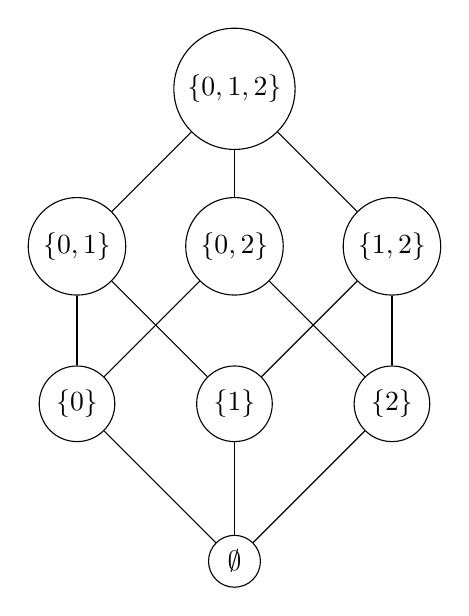
\begin{tikzpicture}[every loop/.style={}]
	
	\node[shape=circle,draw=black] (a) at (2, 0)     {\textbf{$\emptyset$}};
	\node[shape=circle,draw=black] (b) at (2, 2)     {\textbf{$\{1\}$}};
	\node[shape=circle,draw=black] (c) at (0, 2)     {\textbf{$\{0\}$}};
	\node[shape=circle,draw=black] (d) at (4, 2)     {\textbf{$\{2\}$}};
	\node[shape=circle,draw=black] (e) at (0, 4)     {\textbf{$\{0,1\}$}};
	\node[shape=circle,draw=black] (f) at (2, 4)     {\textbf{$\{0,2\}$}};
	\node[shape=circle,draw=black] (g) at (4, 4)     {\textbf{$\{1,2\}$}};
	\node[shape=circle,draw=black] (h) at (2, 6)     {\textbf{$\{0,1,2\}$}};

	
	
	\path[-] (a) edge (b);
	\path[-] (a) edge (c);
	\path[-] (a) edge (d);
	\path[-] (b) edge (e);
	\path[-] (b) edge (g);
	\path[-] (c) edge (e);
	\path[-] (c) edge (f);
	\path[-] (d) edge (f);
	\path[-] (d) edge (g);
	\path[-] (e) edge (h);
	\path[-] (f) edge (h);
	\path[-] (g) edge (h);


	
	\end{tikzpicture} 
	\begin{center}
		Maximal elements: $\{0,1,2\}$\\
		Minimal elements: $\emptyset$
	\end{center}
\end{figure}
\subsection*{e)}
Since we have proved that (S,R) is a poset in the b part, inorder to show (S,R) is lattice it is enough to show that every pair of elements of S has both a least upper bound and greatest lower bound. Pair of elements and their least upper bounds and greatest lower bounds can be seen below;\\
\begin{table}[H]
	\centering
	\vspace{5px}
	\begin{tabular}{|c|c|c|}
		\hline
		Pair&L.U.B&G.L.B\\ \hline
		$\emptyset$ and $\{0\}$&$\{0\}$&$\emptyset$\\ \hline
		$\emptyset$ and $\{1\}$&$\{1\}$&$\emptyset$\\ \hline
		$\emptyset$ and $\{2\}$&$\{2\}$&$\emptyset$\\ \hline
		$\emptyset$ and $\{0,1\}$&$\{0,1\}$&$\emptyset$\\ \hline
		$\emptyset$ and $\{1,2\}$&$\{1,2\}$&$\emptyset$\\ \hline
		$\emptyset$ and $\{0,2\}$&$\{0,2\}$&$\emptyset$\\ \hline
		$\emptyset$ and $\{0,1,2\}$&$\{0,1,2\}$&$\emptyset$\\ \hline
		$\{0\}$and $\{1\}$&$\{0,1\}$&$\emptyset$\\ \hline
		$\{0\}$and $\{2\}$&$\{0,2\}$&$\emptyset$\\ \hline
		$\{0\}$and$\{0,1\}$&$\{0,1\}$&$\{0\}$\\ \hline
		$\{0\}$and$\{1,2\}$&$\{0,1,2\}$&$\emptyset$\\ \hline
		$\{0\}$and$\{0,2\}$&$\{0,2\}$&$\{0\}$\\ \hline
		$\{0\}$and$\{0,1,2\}$&$\{0,1,2\}$&$\{0\}$\\ \hline
		$\{1\}$and $\{2\}$&$\{1,2\}$&$\emptyset$\\ \hline
		$\{1\}$and $\{0,1\}$&$\{0,1\}$&$\{1\}$\\ \hline
		$\{1\}$and $\{0,2\}$&$\{0,1,2\}$&$\emptyset$\\ \hline
		$\{1\}$and $\{1,2\}$&$\{1,2\}$&$\{1\}$\\ \hline
		$\{1\}$and $\{0,1,2\}$&$\{0,1,2\}$&$\{1\}$\\ \hline
		$\{2\}$and$\{0,1\}$&$\{0,1,2\}$&$\emptyset$\\ \hline
		$\{2\}$and$\{1,2\}$&$\{1,2\}$&$\{2\}$\\ \hline
		$\{2\}$and$\{0,2\}$&$\{0,2\}$&$\{2\}$\\ \hline
		$\{2\}$and$\{0,1,2\}$&$\{0,1,2\}$&$\{2\}$\\ \hline
		$\{0,1\}$and$\{1,2\}$&$\{0,1,2\}$&$\{1\}$\\ \hline
		$\{0,1\}$and$\{0,2\}$&$\{0,1,2\}$&$\{0\}$\\ \hline
		$\{0,1\}$and$\{0,1,2\}$&$\{0,1,2\}$&$\{0,1\}$\\ \hline
		$\{0,2\}$and$\{1,2\}$&$\{0,1,2\}$&$\{2\}$\\ \hline
		$\{0,2\}$and$\{0,1,2\}$&$\{0,1,2\}$&$\{0,2\}$\\ \hline
		$\{1,2\}$and$\{0,1,2\}$&$\{0,1,2\}$&$\{1,2\}$\\ \hline
		$\emptyset$and$\emptyset$&$\emptyset$&$\emptyset$\\ \hline
		$\{0\}$and$\{0\}$&$\{0\}$&$\{0\}$\\ \hline
		$\{1\}$and$\{1\}$&$\{1\}$&$\{1\}$\\ \hline
		$\{2\}$and$\{2\}$&$\{2\}$&$\{2\}$\\ \hline
		$\{0,1\}$and$\{0,1\}$&$\{0,1\}$&$\{0,1\}$\\ \hline
		$\{1,2\}$and$\{1,2\}$&$\{1,2\}$&$\{1,2\}$\\ \hline
		$\{0,2\}$and$\{0,2\}$&$\{0,2\}$&$\{0,2\}$\\ \hline
		$\{0,1,2\}$and$\{0,1,2\}$&$\{0,1,2\}$&$\{0,1,2\}$\\ \hline
	\end{tabular}
\end{table}  
By looking the table above, we can easily seen that every pair of elements of S has both least upper bound and greatest lower bound. Additionally, by looking the table above, it can be easily seen that for arbitrarily chosen $x,y\in S$ least upper bound of x and y equal to $x \cup y $ while the greatest lower bound of x and y equal to $x \cap y$. Since we are able to find least upper bound and greatest lower bound for every pair of elements of S, we have showed that (S,R) is a lattice.

\section*{Answer 2}
\subsection*{a)}
\begin{table}[H]
	\centering
	\vspace{5px}
	\begin{tabular}{|c|c|}
		\hline
		Initial Vertex&Terminal Vertices\\ \hline
		a&\\ \hline
		b&a, c\\ \hline
		c&f\\ \hline
		d&a, c, d, e, g\\ \hline
		e&c, f, g\\ \hline
		f&b\\ \hline
		g&d\\ \hline
	\end{tabular}
\end{table}  
\subsection*{b)}
Rows and columns are ordered as a,b,c,d,e,f,g \\
$
\begin{bmatrix}
	0 & 0 & 0 & 0 & 0 & 0 & 0\\
	1 & 0 & 1 & 0 & 0 & 0 & 0\\
	0 & 0 & 0 & 0 & 0 & 1 & 0\\
	1 & 0 & 1 & 1 & 1 & 0 & 1\\
	0 & 0 & 1 & 0 & 0 & 1 & 1\\
	0 & 1 & 0 & 0 & 0 & 0 & 0\\
	0 & 0 & 0 & 1 & 0 & 0 & 0\\
\end{bmatrix}
$
\subsection*{c)}
$
deg^{-}(a) = 2\\
deg^{+}(a) = 0\\
deg^{-}(b) = 1\\
deg^{+}(b) = 2\\
deg^{-}(c) = 3\\
deg^{+}(c) = 1\\
deg^{-}(d) = 2\\
deg^{+}(d) = 5\\
deg^{-}(e) = 1\\
deg^{+}(e) = 3\\
deg^{-}(f) = 2\\
deg^{+}(f) = 1\\
deg^{-}(g) = 2\\
deg^{+}(g) = 1
$
\subsection*{d)}
e,c,f,b,a \\
d,e,f,b,a \\
d,c,f,b,a \\
e,g,d,c,f \\
d,e,f,b,c \\
g,d,c,f,b 
\subsection*{e)}
c,f,b,c \\
d,e,g,d \\
d,g,d,d \\
f,b,c,f \\
b,c,f,b \\
e,g,d,e \\
g,d,e,g \\
g,d,d,g \\
d,d,g,d \\

\subsection*{f)}
To prove that G is weakly connected, we need to show that there is a path between every two distinct vertices in the underlying undirected graph. All possible distinct vertex pairs of G and paths between those vertex pairs can be seen from the table below; \\
\begin{table}[H]
	\centering
	\vspace{5px}
	\begin{tabular}{|c|c|}
		\hline
		Vertex Pairs & Paths  \\ \hline
		a and b&$a,b$\\ \hline
		a and c&$a,b,c$\\ \hline
		a and d&$a,d$\\ \hline
		a and e&$a,d,e$\\ \hline
		a and f&$a,d,e,f$\\ \hline
		a and g&$a,d,e,g$\\ \hline
		b and c&$b,c$\\ \hline
		b and d&$b,c,d$\\ \hline
		b and e&$b,c,e$\\ \hline
		b and f&$b,f$\\ \hline
		b and g&$b,c,e,g$\\ \hline
		c and d&$c,d$\\ \hline
		c and e&$c,e$\\ \hline
		c and f&$c,f$\\ \hline
		c and g&$c,e,g$\\ \hline
		d and e&$d,e$\\ \hline
		d and f&$d,e,f$\\ \hline
		d and g&$d,e,g$\\ \hline
		e and f&$e,f$\\ \hline
		e and g&$e,g$\\ \hline
		f and g&$f,e,g$\\ \hline
	\end{tabular}
\end{table}  
Hence, by observing the table given above, we have proved that there exists a path between every two distinct vertices in the underlying undirected graph. Thus, by the definition G is weakly connected.

\subsection*{g)}
$\{a\}, \{b,c,f\}, \{d,e,g\}$
\subsection*{h)}
Let adjacency matrix of H be A where A is, \\
(Rows and columns are ordered as d,e,f,g) \\
$
\begin{bmatrix}
1 & 1 & 0 & 1 \\
0 & 0 & 1 & 1 \\
0 & 0 & 0 & 0 \\
1 & 0 & 0 & 0 \\
\end{bmatrix}
$\\ \\
To find number of different paths of length 3 from $d$ to $g$ in H, we can use the THEOREM2 placed in Rosen's Discrete Mathematics and Its Applications book page 688. Then by using matrix multiplication we should find the $A^{3}$,
\begin{equation*}
\begin{split}
A^{3} = \begin{bmatrix}
4 & 2 & 1 & 3 \\
1 & 1 & 0 & 1 \\
0 & 0 & 0 & 0 \\
2 & 1 & 1 & 2 \\
\end{bmatrix}
\end{split}
\end{equation*}
Then, by using to theorem mentioned above, number of different paths of length 3 from $d$ to $g$ in H which is represented as $N$,
\begin{equation*}
\begin{split}
N = \ (1,4)th \ entry \ of \ A^{3} \ = 3
\end{split}
\end{equation*}
Thus, number of different paths of length 3 from $d$ to $g$ in H is 3.


\section*{Answer 3}
Firstly, let we entitle each edge of G as, \\
\begin{figure}[H]
	\centering
	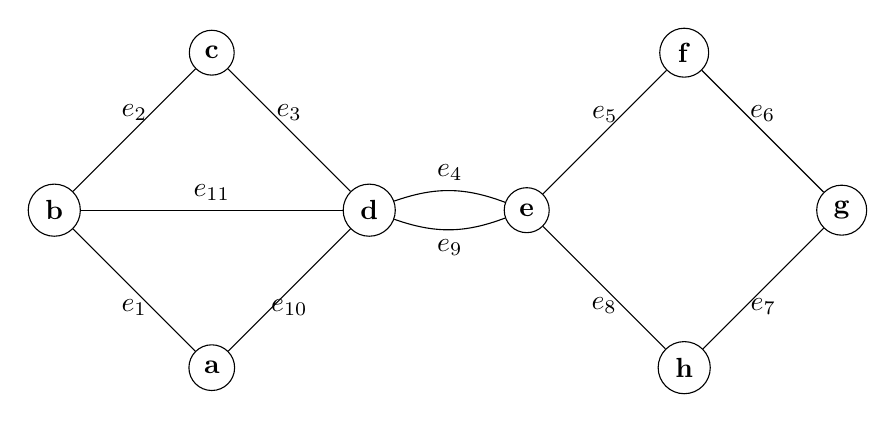
\begin{tikzpicture}[every loop/.style={}]
	
	\node[shape=circle,draw=black] (a) at (2, 0)     {\textbf{a}};
	\node[shape=circle,draw=black] (b) at (0, 2)     {\textbf{b}};
	\node[shape=circle,draw=black] (c) at (2, 4)     {\textbf{c}};
	\node[shape=circle,draw=black] (d) at (4, 2)     {\textbf{d}};
	\node[shape=circle,draw=black] (e) at (6, 2)     {\textbf{e}};
	\node[shape=circle,draw=black] (f) at (8, 4)     {\textbf{f}};
	\node[shape=circle,draw=black] (g) at (10, 2)     {\textbf{g}};
	\node[shape=circle,draw=black] (h) at (8, 0)     {\textbf{h}};
	
	
	\path[-] (b) edge node[above]{$e_{2}$} (c);
	\path[-] (b) edge node[below]{$e_{1}$} (a);
	\path[-] (b) edge node[above]{$e_{11}$} (d);
	\path[-] (c) edge node[above]{$e_{3}$} (d);
	\path[-] (a) edge node[below]{$e_{10}$} (d);
	\path[-] (d) edge [bend left=20] node[above] {$e_{4}$} (e);
	\path[-] (e) edge [bend left=20] node[below] {$e_{9}$} (d);
	\path[-] (e) edge node[above]{$e_{5}$} (f);
	\path[-] (e) edge node[below]{$e_{8}$} (h);
	\path[-] (f) edge node[above]{$e_{6}$} (g);
	\path[-] (h) edge node[below]{$e_{7}$} (g);
	
	\end{tikzpicture} 
	\caption{G}
\end{figure}
\subsection*{a)}
Since the path which can be represented as $e_{1}$, $e_{10}$, $e_{11}$, $e_{2}$, $e_{3}$, $e_{4}$, $e_{5}$, $e_{6}$, $e_{7}$, $e_{8}$, $e_{9}$ doesn't contain the same edge more than once, by the definition given path is a simple path. Moreover, since the given path is simple and containing every edge of G then by the definition, the given path is an Euler Path. Thus, we have proved that G has an Euler Path.
\subsection*{b)}
Since G is an undirected graph and we can find a path between every pair of distinct vertices of G, then by the definition G is a connected graph. Since G is a connected multigraph then we can use the THEOREM 1 placed in the Rosen's Discrete Mathematics and Its Applications book page 696. Assume G has a Euler circuit then by the given theorem we can conclude that each vertices of G must have even degree. However, degree of $b$ is 3 which is not an even degree. Since this fact contradicts with our assumption, by using proof by contradiction we have proved that G doesn't have any Euler circuit.

\subsection*{c)}
Since the path which can be represented as $e_{1}$, $e_{2}$, $e_{3}$, $e_{4}$, $e_{5}$, $e_{6}$, $e_{7}$ doesn't contain the same edge more than once, by the definition given path is a simple path. Moreover, since the given path is simple and passes through every vertex of G exactly once then by the definition given path is a Hamiltonian Path. Thus, we have proved that G has a Hamiltonian Path.
\subsection*{d)}
Since the degrees of $a,c,h,f$ are equal to 2, every possible circuits that include all vertices of G must have $e_{2},e_{3},e_{1},e_{10},e_{5},e_{6},e_{7},e_{8}$ edges. Let's assume that G has a Hamiltonian Circuit, then by the definition, the hamiltonian circuit of G must pass through every vertex exactly once. Since every possible circuits that include all vertices of G must have $e_{2},e_{3},e_{1},e_{10},e_{5},e_{6},e_{7},e_{8}$ edges, then the Hamiltonian Circuit of G must also have $e_{2},e_{3},e_{1},e_{10},e_{5},e_{6},e_{7},e_{8}$ edges. However, since one of the endpoints of $e_{3}$, $e_{10}$, $e_{5}$ and $e_{8}$ is $d$, there isn't any circuit that include all vertices of G and pass through $d$ exactly once. Since this fact contradicts with our assumption, by using the proof by contradiction, G doesn't have any Hamiltonian Circuit.

\section*{Answer 4}
Firstly, let $V = \{a,b,c,d,e\}$ for $G=(V,E)$ and $V'= \{a',b',c',d',e'\}$ for $G'=(V',E')$ also we know that both $G$ and $G'$ are simple graphs.If we can find a one to one and onto $f$ function where $f:V \rightarrow V'$ such that $x$ and $y$ vertices are adjacent in $G$ if and only if $f(x)$ and $f(y)$ are adjacent in $G'$, then by the definition we can prove that $G$ and $G'$ are isomorphic. \\
Let $f:V \rightarrow V'$ be a one to one and onto function such that, 
\begin{equation*}
f(a) = a', \qquad
f(b) = b', \qquad
f(c) = c', \qquad
f(d) = d', \qquad
f(e) = e' \qquad
\end{equation*}
Then, we should check that $x$ and $y$ are adjacent in $G$ if and only if $f(x)$ and $f(y)$ are adjacent in $G'$, \\
\begin{table}[H]
	\centering
	\caption{Adjacency Comparison}
	\vspace{5px}
	\label{my-label1}
	\begin{tabular}{|c|c|}
		\hline
		Adjacent Vertices in G&Adjacent Vertices in G'\\ \hline
		a and b are adjacent&f(a)=a' and f(b)=b' are adjacent\\ \hline
		a and e are adjacent&f(a)=a' and f(e)=e' are adjacent\\ \hline
		b and c are adjacent&f(b)=b' and f(c)=c' are adjacent\\ \hline
		c and d are adjacent&f(c)=c' and f(d)=d' are adjacent\\ \hline
		d and e are adjacent&f(d)=d' and f(e)=e' are adjacent\\ \hline
	\end{tabular}
\end{table}  
By observing Table 1, we can easily see that for all $x$ and $y$ where $x$ and $y$
are vertices in G, if $x$ and $y$ are adjacent then $f(x)=x'$ and $f(y)=y'$ are adjacent in $G'$. Moreover, for all $f(x)=x'$ and $f(y)=y'$ where $x'$ and $y'$ are vertices in $G'$, if $f(x)=x'$ and $f(y)=y'$ adjacent, then $x$ and $y$ are adjacent in $G$. Hence, we have proved that there exist a one to one and onto f function where $f:V \rightarrow V'$ such that $x$ and $y$ vertices are adjacent in $G$ if and only if $f(x)$ and $f(y)$ are adjacent in $G'$. Thus, by the definition, we have proved that $G$ and $G'$ are isomorphic.

\section*{Answer 5}
\subsection*{a)}
We will start from the vertex $a$ and initialize it with distance 0. All other vertices will be initialized with infinite distances. In each step, we will choose the unvisited vertex with the lowest distance as our visited vertex ($v$) and update the distance value of each $u$ vertex adjacent to $v$ as $dist(v)+weight(v,u)$ if $dist(v)+weight(v,u)<dist(u)$.In each step, visited nodes represented with red color, current distance values and current shortest paths from $a$ to each node can be seen from the tables. When we visit the $j$ and color it to red that means we found the shortest distance and the path placed in the table is the shortest path from $a$ to $j$.
\begin{figure}[H]
	\centering
	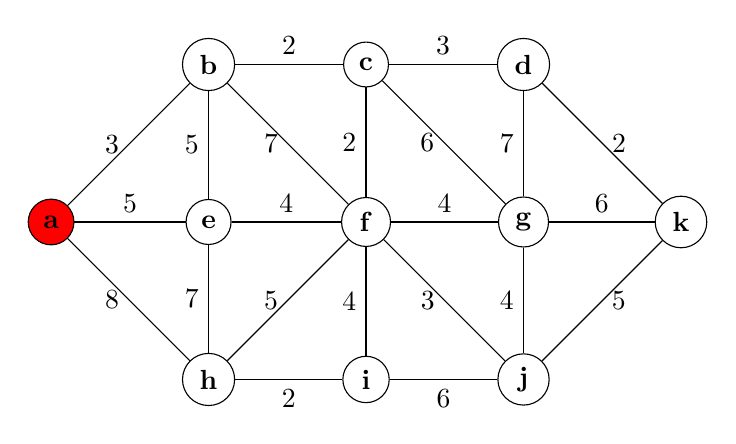
\begin{tikzpicture}
	\node[shape=circle,draw=black, fill = red] (a) at (0, 2)     {\textbf{a}};
	\node[shape=circle,draw=black] (b) at (2, 4)     {\textbf{b}};
	\node[shape=circle,draw=black] (c) at (4, 4)     {\textbf{c}};
	\node[shape=circle,draw=black] (d) at (6, 4)     {\textbf{d}};
	\node[shape=circle,draw=black] (e) at (2, 2)     {\textbf{e}};
	\node[shape=circle,draw=black] (f) at (4, 2)     {\textbf{f}};
	\node[shape=circle,draw=black] (g) at (6, 2)     {\textbf{g}};
	\node[shape=circle,draw=black] (h) at (2, 0)     {\textbf{h}};
	\node[shape=circle,draw=black] (i) at (4, 0)     {\textbf{i}};
	\node[shape=circle,draw=black] (j) at (6, 0)     {\textbf{j}};
	\node[shape=circle,draw=black] (k) at (8, 2)     {\textbf{k}};
	
	\path[-] (a) edge node[left]{3} (b);
	\path[-] (a) edge node[above]{5} (e);
	\path[-] (a) edge node[left]{8} (h);
	\path[-] (b) edge node[left]{5} (e);
	\path[-] (b) edge node[left]{7} (f);
	\path[-] (b) edge node[above]{2} (c);
	\path[-] (e) edge node[above]{4} (f);
	\path[-] (e) edge node[left]{7} (h);
	\path[-] (h) edge node[left]{5} (f);	
	\path[-] (h) edge node[below]{2} (i);	
	\path[-] (c) edge node[above]{3} (d);
	\path[-] (c) edge node[left]{6} (g);
	\path[-] (c) edge node[left]{2} (f);
	\path[-] (f) edge node[above]{4} (g);
	\path[-] (f) edge node[left]{3} (j);
	\path[-] (f) edge node[left]{4} (i);
	\path[-] (i) edge node[below]{6} (j);	
	\path[-] (d) edge node[right]{2} (k);
	\path[-] (d) edge node[left]{7} (g);
	\path[-] (g) edge node[above]{6} (k);
	\path[-] (g) edge node[left]{4} (j);
	\path[-] (j) edge node[right]{5} (k);
	
	\end{tikzpicture} 
\end{figure}
\begin{table}[H]
	\centering
	\vspace{5px}
	\begin{tabular}{|c|c|c|}
		\hline
		Vertex&Distance&Path \\ \hline
		a&0&\\ \hline
		b&3&a,b\\ \hline
		c&inf&\\ \hline
		d&inf&\\ \hline
		e&5&a,e \\ \hline
		f&inf&\\ \hline
		g&inf&\\ \hline
		h&8&a,h\\ \hline
		i&inf&\\ \hline
		j&inf&\\ \hline
		k&inf&\\ \hline
	\end{tabular}
\end{table}  
Since $b$ is the unvisited vertex with the lowest distance, choose it as next visited vertex. \\
\begin{figure}[H]
	\centering
	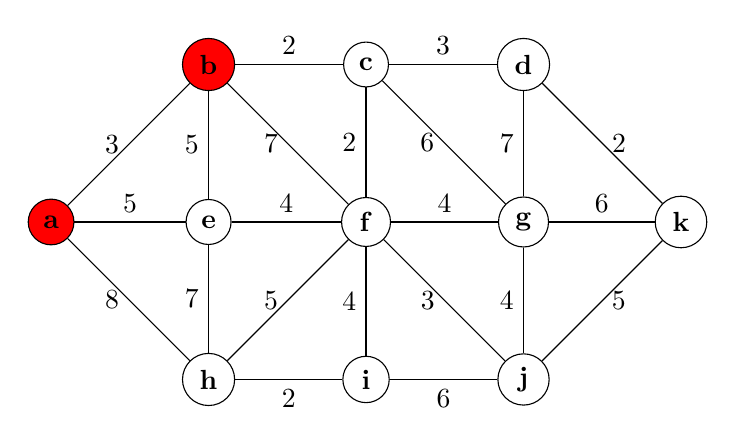
\begin{tikzpicture}
	\node[shape=circle,draw=black, fill = red] (a) at (0, 2)     {\textbf{a}};
	\node[shape=circle,draw=black, fill = red] (b) at (2, 4)     {\textbf{b}};
	\node[shape=circle,draw=black] (c) at (4, 4)     {\textbf{c}};
	\node[shape=circle,draw=black] (d) at (6, 4)     {\textbf{d}};
	\node[shape=circle,draw=black] (e) at (2, 2)     {\textbf{e}};
	\node[shape=circle,draw=black] (f) at (4, 2)     {\textbf{f}};
	\node[shape=circle,draw=black] (g) at (6, 2)     {\textbf{g}};
	\node[shape=circle,draw=black] (h) at (2, 0)     {\textbf{h}};
	\node[shape=circle,draw=black] (i) at (4, 0)     {\textbf{i}};
	\node[shape=circle,draw=black] (j) at (6, 0)     {\textbf{j}};
	\node[shape=circle,draw=black] (k) at (8, 2)     {\textbf{k}};
	
	\path[-] (a) edge node[left]{3} (b);
	\path[-] (a) edge node[above]{5} (e);
	\path[-] (a) edge node[left]{8} (h);
	\path[-] (b) edge node[left]{5} (e);
	\path[-] (b) edge node[left]{7} (f);
	\path[-] (b) edge node[above]{2} (c);
	\path[-] (e) edge node[above]{4} (f);
	\path[-] (e) edge node[left]{7} (h);
	\path[-] (h) edge node[left]{5} (f);	
	\path[-] (h) edge node[below]{2} (i);	
	\path[-] (c) edge node[above]{3} (d);
	\path[-] (c) edge node[left]{6} (g);
	\path[-] (c) edge node[left]{2} (f);
	\path[-] (f) edge node[above]{4} (g);
	\path[-] (f) edge node[left]{3} (j);
	\path[-] (f) edge node[left]{4} (i);
	\path[-] (i) edge node[below]{6} (j);	
	\path[-] (d) edge node[right]{2} (k);
	\path[-] (d) edge node[left]{7} (g);
	\path[-] (g) edge node[above]{6} (k);
	\path[-] (g) edge node[left]{4} (j);
	\path[-] (j) edge node[right]{5} (k);
	
	\end{tikzpicture} 
\end{figure}
\begin{table}[H]
	\centering
	\vspace{5px}
	\begin{tabular}{|c|c|c|}
		\hline
		Vertex&Distance&Path \\ \hline
		a&0&\\ \hline
		b&3&a,b\\ \hline
		c&5&a,b,c\\ \hline
		d&inf&\\ \hline
		e&5&a,e \\ \hline
		f&10&a,b,f\\ \hline
		g&inf&\\ \hline
		h&8&a,h\\ \hline
		i&inf&\\ \hline
		j&inf&\\ \hline
		k&inf&\\ \hline
	\end{tabular}
\end{table}  
Both $c$ and $e$ has same and the lowest distances. So I choose $c$ as the next visited vertex. \\
\begin{figure}[H]
	\centering
	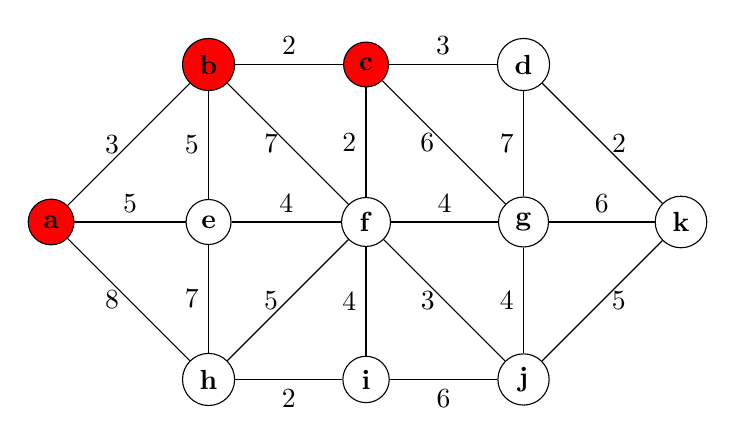
\begin{tikzpicture}
	\node[shape=circle,draw=black, fill = red] (a) at (0, 2)     {\textbf{a}};
	\node[shape=circle,draw=black, fill = red] (b) at (2, 4)     {\textbf{b}};
	\node[shape=circle,draw=black, fill = red] (c) at (4, 4)     {\textbf{c}};
	\node[shape=circle,draw=black] (d) at (6, 4)     {\textbf{d}};
	\node[shape=circle,draw=black] (e) at (2, 2)     {\textbf{e}};
	\node[shape=circle,draw=black] (f) at (4, 2)     {\textbf{f}};
	\node[shape=circle,draw=black] (g) at (6, 2)     {\textbf{g}};
	\node[shape=circle,draw=black] (h) at (2, 0)     {\textbf{h}};
	\node[shape=circle,draw=black] (i) at (4, 0)     {\textbf{i}};
	\node[shape=circle,draw=black] (j) at (6, 0)     {\textbf{j}};
	\node[shape=circle,draw=black] (k) at (8, 2)     {\textbf{k}};
	
	\path[-] (a) edge node[left]{3} (b);
	\path[-] (a) edge node[above]{5} (e);
	\path[-] (a) edge node[left]{8} (h);
	\path[-] (b) edge node[left]{5} (e);
	\path[-] (b) edge node[left]{7} (f);
	\path[-] (b) edge node[above]{2} (c);
	\path[-] (e) edge node[above]{4} (f);
	\path[-] (e) edge node[left]{7} (h);
	\path[-] (h) edge node[left]{5} (f);	
	\path[-] (h) edge node[below]{2} (i);	
	\path[-] (c) edge node[above]{3} (d);
	\path[-] (c) edge node[left]{6} (g);
	\path[-] (c) edge node[left]{2} (f);
	\path[-] (f) edge node[above]{4} (g);
	\path[-] (f) edge node[left]{3} (j);
	\path[-] (f) edge node[left]{4} (i);
	\path[-] (i) edge node[below]{6} (j);	
	\path[-] (d) edge node[right]{2} (k);
	\path[-] (d) edge node[left]{7} (g);
	\path[-] (g) edge node[above]{6} (k);
	\path[-] (g) edge node[left]{4} (j);
	\path[-] (j) edge node[right]{5} (k);
	
	\end{tikzpicture} 
\end{figure}
\begin{table}[H]
	\centering
	\vspace{5px}
	\begin{tabular}{|c|c|c|}
		\hline
		Vertex&Distance&Path \\ \hline
		a&0&\\ \hline
		b&3&a,b\\ \hline
		c&5&a,b,c\\ \hline
		d&8&a,b,c,d\\ \hline
		e&5&a,e \\ \hline
		f&7&a,b,c,f\\ \hline
		g&11&a,b,c,g\\ \hline
		h&8&a,h\\ \hline
		i&inf&\\ \hline
		j&inf&\\ \hline
		k&inf&\\ \hline
	\end{tabular}
\end{table}  
$e$ is the unvisited vertex with the lowest distance. So choose $e$ as the next visited vertex. \\
\begin{figure}[H]
	\centering
	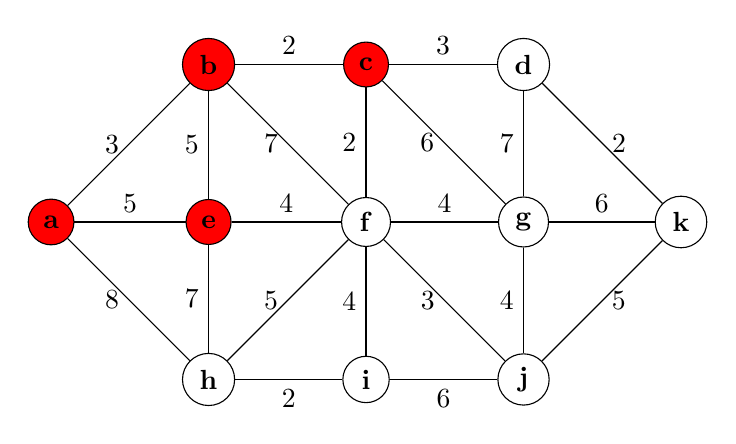
\begin{tikzpicture}
	\node[shape=circle,draw=black, fill = red] (a) at (0, 2)     {\textbf{a}};
	\node[shape=circle,draw=black, fill = red] (b) at (2, 4)     {\textbf{b}};
	\node[shape=circle,draw=black, fill = red] (c) at (4, 4)     {\textbf{c}};
	\node[shape=circle,draw=black] (d) at (6, 4)     {\textbf{d}};
	\node[shape=circle,draw=black, fill = red] (e) at (2, 2)     {\textbf{e}};
	\node[shape=circle,draw=black] (f) at (4, 2)     {\textbf{f}};
	\node[shape=circle,draw=black] (g) at (6, 2)     {\textbf{g}};
	\node[shape=circle,draw=black] (h) at (2, 0)     {\textbf{h}};
	\node[shape=circle,draw=black] (i) at (4, 0)     {\textbf{i}};
	\node[shape=circle,draw=black] (j) at (6, 0)     {\textbf{j}};
	\node[shape=circle,draw=black] (k) at (8, 2)     {\textbf{k}};
	
	\path[-] (a) edge node[left]{3} (b);
	\path[-] (a) edge node[above]{5} (e);
	\path[-] (a) edge node[left]{8} (h);
	\path[-] (b) edge node[left]{5} (e);
	\path[-] (b) edge node[left]{7} (f);
	\path[-] (b) edge node[above]{2} (c);
	\path[-] (e) edge node[above]{4} (f);
	\path[-] (e) edge node[left]{7} (h);
	\path[-] (h) edge node[left]{5} (f);	
	\path[-] (h) edge node[below]{2} (i);	
	\path[-] (c) edge node[above]{3} (d);
	\path[-] (c) edge node[left]{6} (g);
	\path[-] (c) edge node[left]{2} (f);
	\path[-] (f) edge node[above]{4} (g);
	\path[-] (f) edge node[left]{3} (j);
	\path[-] (f) edge node[left]{4} (i);
	\path[-] (i) edge node[below]{6} (j);	
	\path[-] (d) edge node[right]{2} (k);
	\path[-] (d) edge node[left]{7} (g);
	\path[-] (g) edge node[above]{6} (k);
	\path[-] (g) edge node[left]{4} (j);
	\path[-] (j) edge node[right]{5} (k);
	
	\end{tikzpicture} 
\end{figure}
\begin{table}[H]
	\centering
	\vspace{5px}
	\begin{tabular}{|c|c|c|}
		\hline
		Vertex&Distance&Path \\ \hline
		a&0&\\ \hline
		b&3&a,b\\ \hline
		c&5&a,b,c\\ \hline
		d&8&a,b,c,d\\ \hline
		e&5&a,e \\ \hline
		f&7&a,b,c,f\\ \hline
		g&11&a,b,c,g\\ \hline
		h&8&a,h\\ \hline
		i&inf&\\ \hline
		j&inf&\\ \hline
		k&inf&\\ \hline
	\end{tabular}
\end{table}  
$f$ is the unvisited vertex with the lowest distance. So choose $f$ as the next visited vertex. \\
\begin{figure}[H]
	\centering
	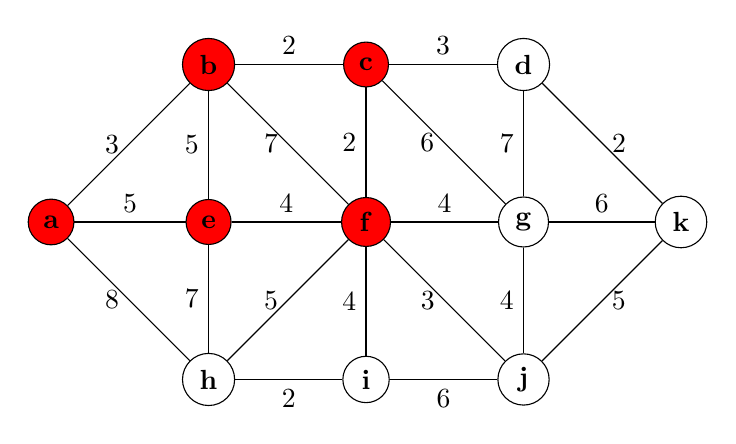
\begin{tikzpicture}
	\node[shape=circle,draw=black, fill = red] (a) at (0, 2)     {\textbf{a}};
	\node[shape=circle,draw=black, fill = red] (b) at (2, 4)     {\textbf{b}};
	\node[shape=circle,draw=black, fill = red] (c) at (4, 4)     {\textbf{c}};
	\node[shape=circle,draw=black] (d) at (6, 4)     {\textbf{d}};
	\node[shape=circle,draw=black, fill = red] (e) at (2, 2)     {\textbf{e}};
	\node[shape=circle,draw=black, fill=red] (f) at (4, 2)     {\textbf{f}};
	\node[shape=circle,draw=black] (g) at (6, 2)     {\textbf{g}};
	\node[shape=circle,draw=black] (h) at (2, 0)     {\textbf{h}};
	\node[shape=circle,draw=black] (i) at (4, 0)     {\textbf{i}};
	\node[shape=circle,draw=black] (j) at (6, 0)     {\textbf{j}};
	\node[shape=circle,draw=black] (k) at (8, 2)     {\textbf{k}};
	
	\path[-] (a) edge node[left]{3} (b);
	\path[-] (a) edge node[above]{5} (e);
	\path[-] (a) edge node[left]{8} (h);
	\path[-] (b) edge node[left]{5} (e);
	\path[-] (b) edge node[left]{7} (f);
	\path[-] (b) edge node[above]{2} (c);
	\path[-] (e) edge node[above]{4} (f);
	\path[-] (e) edge node[left]{7} (h);
	\path[-] (h) edge node[left]{5} (f);	
	\path[-] (h) edge node[below]{2} (i);	
	\path[-] (c) edge node[above]{3} (d);
	\path[-] (c) edge node[left]{6} (g);
	\path[-] (c) edge node[left]{2} (f);
	\path[-] (f) edge node[above]{4} (g);
	\path[-] (f) edge node[left]{3} (j);
	\path[-] (f) edge node[left]{4} (i);
	\path[-] (i) edge node[below]{6} (j);	
	\path[-] (d) edge node[right]{2} (k);
	\path[-] (d) edge node[left]{7} (g);
	\path[-] (g) edge node[above]{6} (k);
	\path[-] (g) edge node[left]{4} (j);
	\path[-] (j) edge node[right]{5} (k);
	
	\end{tikzpicture} 
\end{figure}
\begin{table}[H]
	\centering
	\vspace{5px}
	\begin{tabular}{|c|c|c|}
		\hline
		Vertex&Distance&Path \\ \hline
		a&0&\\ \hline
		b&3&a,b\\ \hline
		c&5&a,b,c\\ \hline
		d&8&a,b,c,d\\ \hline
		e&5&a,e \\ \hline
		f&7&a,b,c,f\\ \hline
		g&11&a,b,c,g\\ \hline
		h&8&a,h\\ \hline
		i&11&a,b,c,f,i\\ \hline
		j&10&a,b,c,f,j\\ \hline
		k&inf&\\ \hline
	\end{tabular}
\end{table}  
Both $d$ and $h$ has same and the lowest distances. So I choose $d$ as the next visited vertex. \\
\begin{figure}[H]
	\centering
	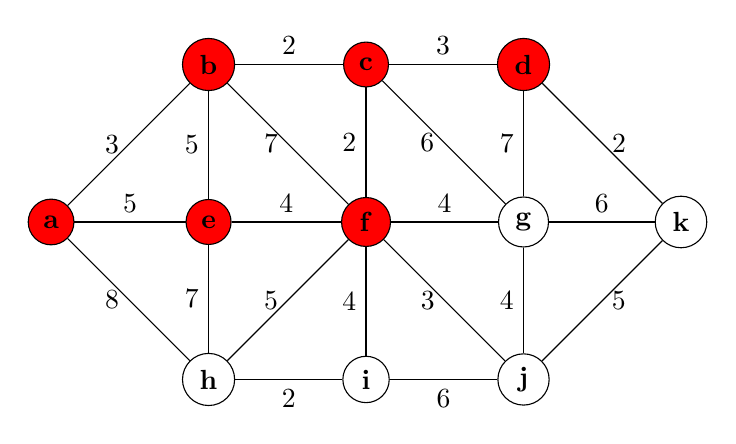
\begin{tikzpicture}
	\node[shape=circle,draw=black, fill = red] (a) at (0, 2)     {\textbf{a}};
	\node[shape=circle,draw=black, fill = red] (b) at (2, 4)     {\textbf{b}};
	\node[shape=circle,draw=black, fill = red] (c) at (4, 4)     {\textbf{c}};
	\node[shape=circle,draw=black,fill=red] (d) at (6, 4)     {\textbf{d}};
	\node[shape=circle,draw=black, fill = red] (e) at (2, 2)     {\textbf{e}};
	\node[shape=circle,draw=black, fill=red] (f) at (4, 2)     {\textbf{f}};
	\node[shape=circle,draw=black] (g) at (6, 2)     {\textbf{g}};
	\node[shape=circle,draw=black] (h) at (2, 0)     {\textbf{h}};
	\node[shape=circle,draw=black] (i) at (4, 0)     {\textbf{i}};
	\node[shape=circle,draw=black] (j) at (6, 0)     {\textbf{j}};
	\node[shape=circle,draw=black] (k) at (8, 2)     {\textbf{k}};
	
	\path[-] (a) edge node[left]{3} (b);
	\path[-] (a) edge node[above]{5} (e);
	\path[-] (a) edge node[left]{8} (h);
	\path[-] (b) edge node[left]{5} (e);
	\path[-] (b) edge node[left]{7} (f);
	\path[-] (b) edge node[above]{2} (c);
	\path[-] (e) edge node[above]{4} (f);
	\path[-] (e) edge node[left]{7} (h);
	\path[-] (h) edge node[left]{5} (f);	
	\path[-] (h) edge node[below]{2} (i);	
	\path[-] (c) edge node[above]{3} (d);
	\path[-] (c) edge node[left]{6} (g);
	\path[-] (c) edge node[left]{2} (f);
	\path[-] (f) edge node[above]{4} (g);
	\path[-] (f) edge node[left]{3} (j);
	\path[-] (f) edge node[left]{4} (i);
	\path[-] (i) edge node[below]{6} (j);	
	\path[-] (d) edge node[right]{2} (k);
	\path[-] (d) edge node[left]{7} (g);
	\path[-] (g) edge node[above]{6} (k);
	\path[-] (g) edge node[left]{4} (j);
	\path[-] (j) edge node[right]{5} (k);
	
	\end{tikzpicture} 
\end{figure}
\begin{table}[H]
	\centering
	\vspace{5px}
	\begin{tabular}{|c|c|c|}
		\hline
		Vertex&Distance&Path \\ \hline
		a&0&\\ \hline
		b&3&a,b\\ \hline
		c&5&a,b,c\\ \hline
		d&8&a,b,c,d\\ \hline
		e&5&a,e \\ \hline
		f&7&a,b,c,f\\ \hline
		g&11&a,b,c,g\\ \hline
		h&8&a,h\\ \hline
		i&11&a,b,c,f,i\\ \hline
		j&10&a,b,c,f,j\\ \hline
		k&10&a,b,c,d,k\\ \hline
	\end{tabular}
\end{table}  
$h$ is the unvisited vertex with the lowest distance. So choose $h$ as the next visited vertex. \\
\begin{figure}[H]
	\centering
	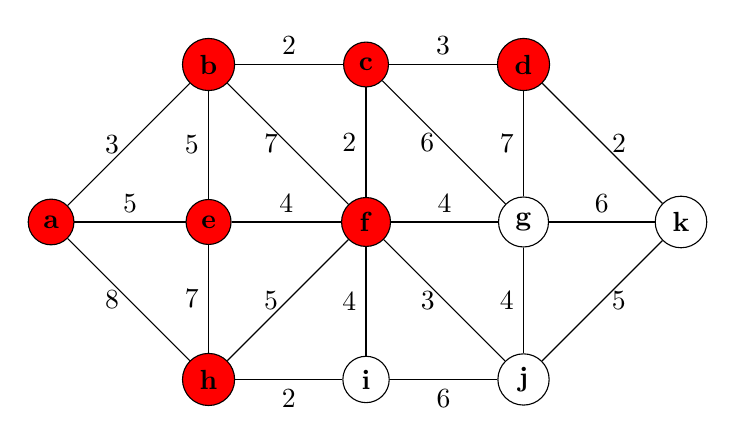
\begin{tikzpicture}
	\node[shape=circle,draw=black, fill = red] (a) at (0, 2)     {\textbf{a}};
	\node[shape=circle,draw=black, fill = red] (b) at (2, 4)     {\textbf{b}};
	\node[shape=circle,draw=black, fill = red] (c) at (4, 4)     {\textbf{c}};
	\node[shape=circle,draw=black,fill=red] (d) at (6, 4)     {\textbf{d}};
	\node[shape=circle,draw=black, fill = red] (e) at (2, 2)     {\textbf{e}};
	\node[shape=circle,draw=black, fill=red] (f) at (4, 2)     {\textbf{f}};
	\node[shape=circle,draw=black] (g) at (6, 2)     {\textbf{g}};
	\node[shape=circle,draw=black,fill=red] (h) at (2, 0)     {\textbf{h}};
	\node[shape=circle,draw=black] (i) at (4, 0)     {\textbf{i}};
	\node[shape=circle,draw=black] (j) at (6, 0)     {\textbf{j}};
	\node[shape=circle,draw=black] (k) at (8, 2)     {\textbf{k}};
	
	\path[-] (a) edge node[left]{3} (b);
	\path[-] (a) edge node[above]{5} (e);
	\path[-] (a) edge node[left]{8} (h);
	\path[-] (b) edge node[left]{5} (e);
	\path[-] (b) edge node[left]{7} (f);
	\path[-] (b) edge node[above]{2} (c);
	\path[-] (e) edge node[above]{4} (f);
	\path[-] (e) edge node[left]{7} (h);
	\path[-] (h) edge node[left]{5} (f);	
	\path[-] (h) edge node[below]{2} (i);	
	\path[-] (c) edge node[above]{3} (d);
	\path[-] (c) edge node[left]{6} (g);
	\path[-] (c) edge node[left]{2} (f);
	\path[-] (f) edge node[above]{4} (g);
	\path[-] (f) edge node[left]{3} (j);
	\path[-] (f) edge node[left]{4} (i);
	\path[-] (i) edge node[below]{6} (j);	
	\path[-] (d) edge node[right]{2} (k);
	\path[-] (d) edge node[left]{7} (g);
	\path[-] (g) edge node[above]{6} (k);
	\path[-] (g) edge node[left]{4} (j);
	\path[-] (j) edge node[right]{5} (k);
	
	\end{tikzpicture} 
\end{figure}
\begin{table}[H]
	\centering
	\vspace{5px}
	\begin{tabular}{|c|c|c|}
		\hline
		Vertex&Distance&Path \\ \hline
		a&0&\\ \hline
		b&3&a,b\\ \hline
		c&5&a,b,c\\ \hline
		d&8&a,b,c,d\\ \hline
		e&5&a,e \\ \hline
		f&7&a,b,c,f\\ \hline
		g&11&a,b,c,g\\ \hline
		h&8&a,h\\ \hline
		i&10&a,h,i\\ \hline
		j&10&a,b,c,f,j\\ \hline
		k&10&a,b,c,d,k\\ \hline
	\end{tabular}
\end{table}  
$i$, $j$ and $k$ has same and the lowest distance value. So I choose $j$ as the next visited vertex. \\
\begin{figure}[H]
	\centering
	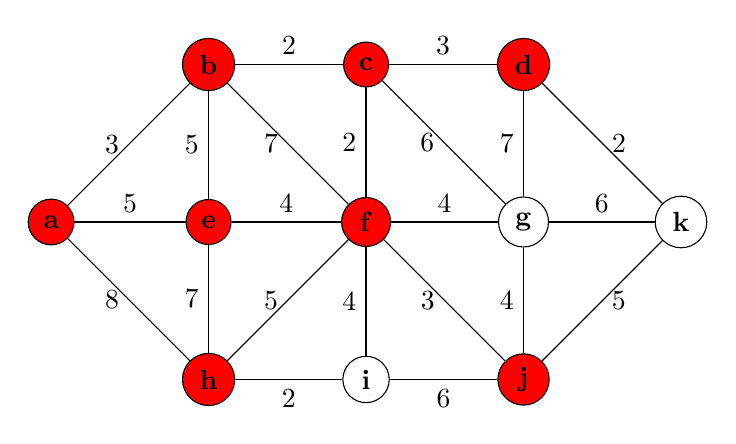
\begin{tikzpicture}
	\node[shape=circle,draw=black, fill = red] (a) at (0, 2)     {\textbf{a}};
	\node[shape=circle,draw=black, fill = red] (b) at (2, 4)     {\textbf{b}};
	\node[shape=circle,draw=black, fill = red] (c) at (4, 4)     {\textbf{c}};
	\node[shape=circle,draw=black,fill=red] (d) at (6, 4)     {\textbf{d}};
	\node[shape=circle,draw=black, fill = red] (e) at (2, 2)     {\textbf{e}};
	\node[shape=circle,draw=black, fill=red] (f) at (4, 2)     {\textbf{f}};
	\node[shape=circle,draw=black] (g) at (6, 2)     {\textbf{g}};
	\node[shape=circle,draw=black,fill=red] (h) at (2, 0)     {\textbf{h}};
	\node[shape=circle,draw=black] (i) at (4, 0)     {\textbf{i}};
	\node[shape=circle,draw=black,fill=red] (j) at (6, 0)     {\textbf{j}};
	\node[shape=circle,draw=black] (k) at (8, 2)     {\textbf{k}};
	
	\path[-] (a) edge node[left]{3} (b);
	\path[-] (a) edge node[above]{5} (e);
	\path[-] (a) edge node[left]{8} (h);
	\path[-] (b) edge node[left]{5} (e);
	\path[-] (b) edge node[left]{7} (f);
	\path[-] (b) edge node[above]{2} (c);
	\path[-] (e) edge node[above]{4} (f);
	\path[-] (e) edge node[left]{7} (h);
	\path[-] (h) edge node[left]{5} (f);	
	\path[-] (h) edge node[below]{2} (i);	
	\path[-] (c) edge node[above]{3} (d);
	\path[-] (c) edge node[left]{6} (g);
	\path[-] (c) edge node[left]{2} (f);
	\path[-] (f) edge node[above]{4} (g);
	\path[-] (f) edge node[left]{3} (j);
	\path[-] (f) edge node[left]{4} (i);
	\path[-] (i) edge node[below]{6} (j);	
	\path[-] (d) edge node[right]{2} (k);
	\path[-] (d) edge node[left]{7} (g);
	\path[-] (g) edge node[above]{6} (k);
	\path[-] (g) edge node[left]{4} (j);
	\path[-] (j) edge node[right]{5} (k);
	
	\end{tikzpicture} 
\end{figure}
\begin{table}[H]
	\centering
	\vspace{5px}
	\begin{tabular}{|c|c|c|}
		\hline
		Vertex&Distance&Path \\ \hline
		a&0&\\ \hline
		b&3&a,b\\ \hline
		c&5&a,b,c\\ \hline
		d&8&a,b,c,d\\ \hline
		e&5&a,e \\ \hline
		f&7&a,b,c,f\\ \hline
		g&11&a,b,c,g\\ \hline
		h&8&a,h\\ \hline
		i&10&a,h,i\\ \hline
		j&10&a,b,c,f,j\\ \hline
		k&10&a,b,c,d,k\\ \hline
	\end{tabular}
\end{table}  
Since we have visited $j$, we have found the shortest path from $a$ to $j$ by applying Dijkstra's Shortest Path Algorithm. According to the table shortest distance between $a$ and $j$ is 10 and the shortest path from $a$ to $j$ is a,b,c,f,j.

\subsection*{b)}
\begin{figure}[H]
	\centering
	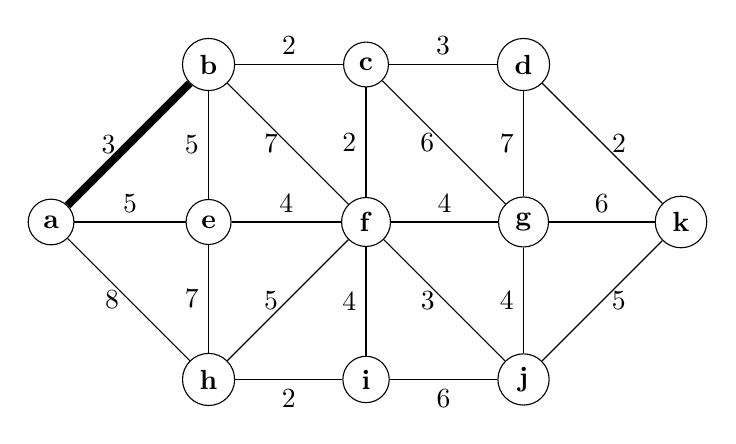
\begin{tikzpicture}
	\node[shape=circle,draw=black] (a) at (0, 2)     {\textbf{a}};
	\node[shape=circle,draw=black] (b) at (2, 4)     {\textbf{b}};
	\node[shape=circle,draw=black] (c) at (4, 4)     {\textbf{c}};
	\node[shape=circle,draw=black] (d) at (6, 4)     {\textbf{d}};
	\node[shape=circle,draw=black] (e) at (2, 2)     {\textbf{e}};
	\node[shape=circle,draw=black] (f) at (4, 2)     {\textbf{f}};
	\node[shape=circle,draw=black] (g) at (6, 2)     {\textbf{g}};
	\node[shape=circle,draw=black] (h) at (2, 0)     {\textbf{h}};
	\node[shape=circle,draw=black] (i) at (4, 0)     {\textbf{i}};
	\node[shape=circle,draw=black] (j) at (6, 0)     {\textbf{j}};
	\node[shape=circle,draw=black] (k) at (8, 2)     {\textbf{k}};
	
	\path[-, line width=1mm] (a) edge node[left]{3} (b);
	\path[-] (a) edge node[above]{5} (e);
	\path[-] (a) edge node[left]{8} (h);
	\path[-] (b) edge node[left]{5} (e);
	\path[-] (b) edge node[left]{7} (f);
	\path[-] (b) edge node[above]{2} (c);
	\path[-] (e) edge node[above]{4} (f);
	\path[-] (e) edge node[left]{7} (h);
	\path[-] (h) edge node[left]{5} (f);	
	\path[-] (h) edge node[below]{2} (i);	
	\path[-] (c) edge node[above]{3} (d);
	\path[-] (c) edge node[left]{6} (g);
	\path[-] (c) edge node[left]{2} (f);
	\path[-] (f) edge node[above]{4} (g);
	\path[-] (f) edge node[left]{3} (j);
	\path[-] (f) edge node[left]{4} (i);
	\path[-] (i) edge node[below]{6} (j);	
	\path[-] (d) edge node[right]{2} (k);
	\path[-] (d) edge node[left]{7} (g);
	\path[-] (g) edge node[above]{6} (k);
	\path[-] (g) edge node[left]{4} (j);
	\path[-] (j) edge node[right]{5} (k);
	\end{tikzpicture} 
	\\
Since we chose $a$ as a root vertex, to apply Prim's rule we should find the edge of minimum weight incident to $a$. Since the weight of ${a,b}$ is smaller than the other edges incident to $a$ and ${a,b}$ doesn't cause a simple circuit on the spanning tree, we should add ${a,b}$ to our spanning tree and $b$ is now visited. \\
\end{figure}

\begin{figure}[H]
	\centering
	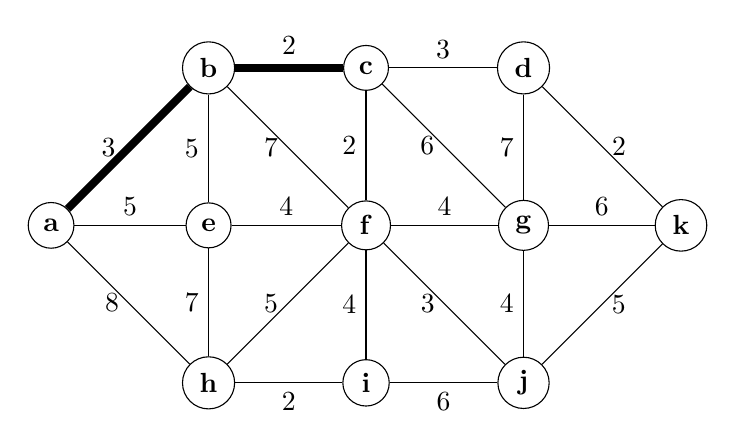
\begin{tikzpicture}
	\node[shape=circle,draw=black] (a) at (0, 2)     {\textbf{a}};
	\node[shape=circle,draw=black] (b) at (2, 4)     {\textbf{b}};
	\node[shape=circle,draw=black] (c) at (4, 4)     {\textbf{c}};
	\node[shape=circle,draw=black] (d) at (6, 4)     {\textbf{d}};
	\node[shape=circle,draw=black] (e) at (2, 2)     {\textbf{e}};
	\node[shape=circle,draw=black] (f) at (4, 2)     {\textbf{f}};
	\node[shape=circle,draw=black] (g) at (6, 2)     {\textbf{g}};
	\node[shape=circle,draw=black] (h) at (2, 0)     {\textbf{h}};
	\node[shape=circle,draw=black] (i) at (4, 0)     {\textbf{i}};
	\node[shape=circle,draw=black] (j) at (6, 0)     {\textbf{j}};
	\node[shape=circle,draw=black] (k) at (8, 2)     {\textbf{k}};
	
	\path[-, line width=1mm] (a) edge node[left]{3} (b);
	\path[-] (a) edge node[above]{5} (e);
	\path[-] (a) edge node[left]{8} (h);
	\path[-] (b) edge node[left]{5} (e);
	\path[-] (b) edge node[left]{7} (f);
	\path[-, line width=1mm] (b) edge node[above]{2} (c);
	\path[-] (e) edge node[above]{4} (f);
	\path[-] (e) edge node[left]{7} (h);
	\path[-] (h) edge node[left]{5} (f);	
	\path[-] (h) edge node[below]{2} (i);	
	\path[-] (c) edge node[above]{3} (d);
	\path[-] (c) edge node[left]{6} (g);
	\path[-] (c) edge node[left]{2} (f);
	\path[-] (f) edge node[above]{4} (g);
	\path[-] (f) edge node[left]{3} (j);
	\path[-] (f) edge node[left]{4} (i);
	\path[-] (i) edge node[below]{6} (j);	
	\path[-] (d) edge node[right]{2} (k);
	\path[-] (d) edge node[left]{7} (g);
	\path[-] (g) edge node[above]{6} (k);
	\path[-] (g) edge node[left]{4} (j);
	\path[-] (j) edge node[right]{5} (k);
	\end{tikzpicture} 
	\\
	${a,h}$, ${a,e}$, ${b,e}$, ${b,f}$ and ${b,c}$ are incident edges to the current vertices which are $a$ and $b$ of our spanning tree. Since the weight of ${b,c}$ is lower than the other incident edges and doesn't cause a simple circuit on the spanning tree, according to Prim's Algorithm we should add ${b,c}$ to our spanning tree and $c$ is now visited.

\end{figure}

\begin{figure}[H]
	\centering
	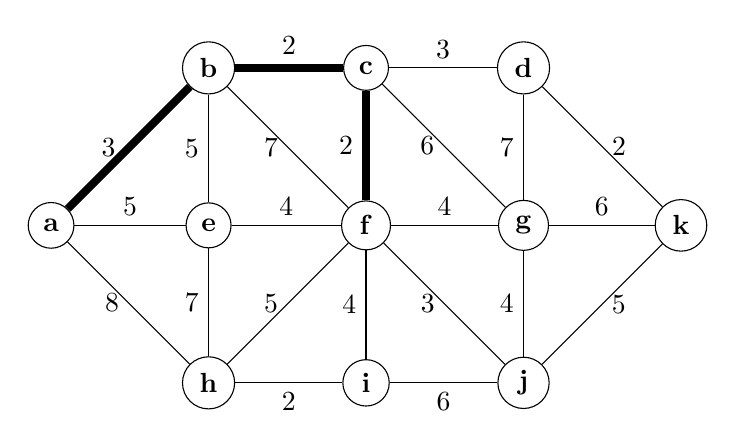
\begin{tikzpicture}
	\node[shape=circle,draw=black] (a) at (0, 2)     {\textbf{a}};
	\node[shape=circle,draw=black] (b) at (2, 4)     {\textbf{b}};
	\node[shape=circle,draw=black] (c) at (4, 4)     {\textbf{c}};
	\node[shape=circle,draw=black] (d) at (6, 4)     {\textbf{d}};
	\node[shape=circle,draw=black] (e) at (2, 2)     {\textbf{e}};
	\node[shape=circle,draw=black] (f) at (4, 2)     {\textbf{f}};
	\node[shape=circle,draw=black] (g) at (6, 2)     {\textbf{g}};
	\node[shape=circle,draw=black] (h) at (2, 0)     {\textbf{h}};
	\node[shape=circle,draw=black] (i) at (4, 0)     {\textbf{i}};
	\node[shape=circle,draw=black] (j) at (6, 0)     {\textbf{j}};
	\node[shape=circle,draw=black] (k) at (8, 2)     {\textbf{k}};
	
	\path[-, line width=1mm] (a) edge node[left]{3} (b);
	\path[-] (a) edge node[above]{5} (e);
	\path[-] (a) edge node[left]{8} (h);
	\path[-] (b) edge node[left]{5} (e);
	\path[-] (b) edge node[left]{7} (f);
	\path[-, line width=1mm] (b) edge node[above]{2} (c);
	\path[-] (e) edge node[above]{4} (f);
	\path[-] (e) edge node[left]{7} (h);
	\path[-] (h) edge node[left]{5} (f);	
	\path[-] (h) edge node[below]{2} (i);	
	\path[-] (c) edge node[above]{3} (d);
	\path[-] (c) edge node[left]{6} (g);
	\path[-, line width=1mm] (c) edge node[left]{2} (f);
	\path[-] (f) edge node[above]{4} (g);
	\path[-] (f) edge node[left]{3} (j);
	\path[-] (f) edge node[left]{4} (i);
	\path[-] (i) edge node[below]{6} (j);	
	\path[-] (d) edge node[right]{2} (k);
	\path[-] (d) edge node[left]{7} (g);
	\path[-] (g) edge node[above]{6} (k);
	\path[-] (g) edge node[left]{4} (j);
	\path[-] (j) edge node[right]{5} (k);
	\end{tikzpicture} 
	\\
	If we control each incident edges to the current vertices our spanning tree has, we can easily see that the one with smallest weight is ${c,f}$ whose weight is 2. Since ${c,f}$ has the smallest weight among the incident edges and doesn't create any simple circuits on the spanning tree according to the Prim's Algorithm we should add ${c,f}$ to our spanning tree.
	
\end{figure}

\begin{figure}[H]
	\centering
	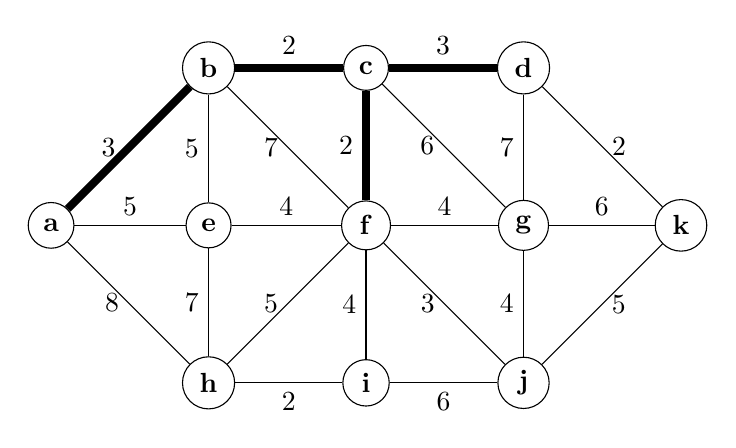
\begin{tikzpicture}
	\node[shape=circle,draw=black] (a) at (0, 2)     {\textbf{a}};
	\node[shape=circle,draw=black] (b) at (2, 4)     {\textbf{b}};
	\node[shape=circle,draw=black] (c) at (4, 4)     {\textbf{c}};
	\node[shape=circle,draw=black] (d) at (6, 4)     {\textbf{d}};
	\node[shape=circle,draw=black] (e) at (2, 2)     {\textbf{e}};
	\node[shape=circle,draw=black] (f) at (4, 2)     {\textbf{f}};
	\node[shape=circle,draw=black] (g) at (6, 2)     {\textbf{g}};
	\node[shape=circle,draw=black] (h) at (2, 0)     {\textbf{h}};
	\node[shape=circle,draw=black] (i) at (4, 0)     {\textbf{i}};
	\node[shape=circle,draw=black] (j) at (6, 0)     {\textbf{j}};
	\node[shape=circle,draw=black] (k) at (8, 2)     {\textbf{k}};
	
	\path[-, line width=1mm] (a) edge node[left]{3} (b);
	\path[-] (a) edge node[above]{5} (e);
	\path[-] (a) edge node[left]{8} (h);
	\path[-] (b) edge node[left]{5} (e);
	\path[-] (b) edge node[left]{7} (f);
	\path[-, line width=1mm] (b) edge node[above]{2} (c);
	\path[-] (e) edge node[above]{4} (f);
	\path[-] (e) edge node[left]{7} (h);
	\path[-] (h) edge node[left]{5} (f);	
	\path[-] (h) edge node[below]{2} (i);	
	\path[- , line width=1mm] (c) edge node[above]{3} (d);
	\path[-] (c) edge node[left]{6} (g);
	\path[-, line width=1mm] (c) edge node[left]{2} (f);
	\path[-] (f) edge node[above]{4} (g);
	\path[-] (f) edge node[left]{3} (j);
	\path[-] (f) edge node[left]{4} (i);
	\path[-] (i) edge node[below]{6} (j);	
	\path[-] (d) edge node[right]{2} (k);
	\path[-] (d) edge node[left]{7} (g);
	\path[-] (g) edge node[above]{6} (k);
	\path[-] (g) edge node[left]{4} (j);
	\path[-] (j) edge node[right]{5} (k);
	\end{tikzpicture} 
	\\
	If we control each incident edges to the current vertices our spanning tree has, we can easily see that both ${c,d}$ and ${f,j}$ has the lowest weight which is 3. Since both ${c,d}$ and ${f,j}$ doesn't create any simple circuits on the spanning tree according to the Prim's Algorithm, we  can add either of them, so that at this point I choose to add ${c,d}$ to our spanning tree.
	
\end{figure}
\begin{figure}[H]
	\centering
	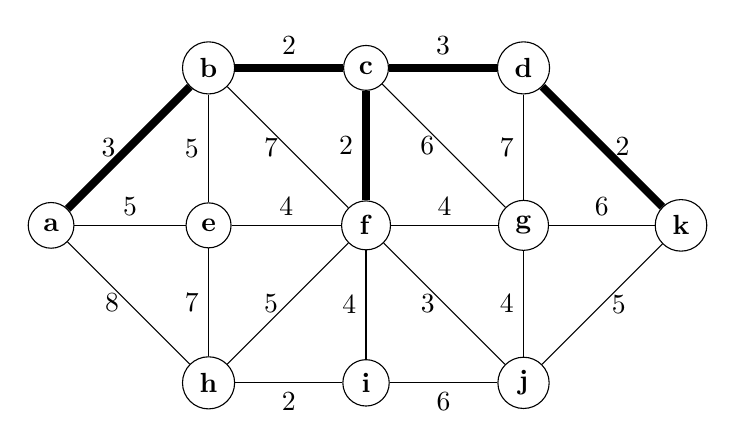
\begin{tikzpicture}
	\node[shape=circle,draw=black] (a) at (0, 2)     {\textbf{a}};
	\node[shape=circle,draw=black] (b) at (2, 4)     {\textbf{b}};
	\node[shape=circle,draw=black] (c) at (4, 4)     {\textbf{c}};
	\node[shape=circle,draw=black] (d) at (6, 4)     {\textbf{d}};
	\node[shape=circle,draw=black] (e) at (2, 2)     {\textbf{e}};
	\node[shape=circle,draw=black] (f) at (4, 2)     {\textbf{f}};
	\node[shape=circle,draw=black] (g) at (6, 2)     {\textbf{g}};
	\node[shape=circle,draw=black] (h) at (2, 0)     {\textbf{h}};
	\node[shape=circle,draw=black] (i) at (4, 0)     {\textbf{i}};
	\node[shape=circle,draw=black] (j) at (6, 0)     {\textbf{j}};
	\node[shape=circle,draw=black] (k) at (8, 2)     {\textbf{k}};
	
	\path[-, line width=1mm] (a) edge node[left]{3} (b);
	\path[-] (a) edge node[above]{5} (e);
	\path[-] (a) edge node[left]{8} (h);
	\path[-] (b) edge node[left]{5} (e);
	\path[-] (b) edge node[left]{7} (f);
	\path[-, line width=1mm] (b) edge node[above]{2} (c);
	\path[-] (e) edge node[above]{4} (f);
	\path[-] (e) edge node[left]{7} (h);
	\path[-] (h) edge node[left]{5} (f);	
	\path[-] (h) edge node[below]{2} (i);	
	\path[- , line width=1mm] (c) edge node[above]{3} (d);
	\path[-] (c) edge node[left]{6} (g);
	\path[-, line width=1mm] (c) edge node[left]{2} (f);
	\path[-] (f) edge node[above]{4} (g);
	\path[-] (f) edge node[left]{3} (j);
	\path[-] (f) edge node[left]{4} (i);
	\path[-] (i) edge node[below]{6} (j);	
	\path[-, line width=1mm] (d) edge node[right]{2} (k);
	\path[-] (d) edge node[left]{7} (g);
	\path[-] (g) edge node[above]{6} (k);
	\path[-] (g) edge node[left]{4} (j);
	\path[-] (j) edge node[right]{5} (k);
	\end{tikzpicture} 
	\\
	If we control each incident edges to the current vertices our spanning tree has, we can easily see that ${d,k}$ has the lowest weight which is 2. Since ${d,k}$ doesn't create any simple circuits on the spanning tree according to the Prim's Algorithm we should add ${d,k}$ to the spanning tree.
	
\end{figure}

\begin{figure}[H]
	\centering
	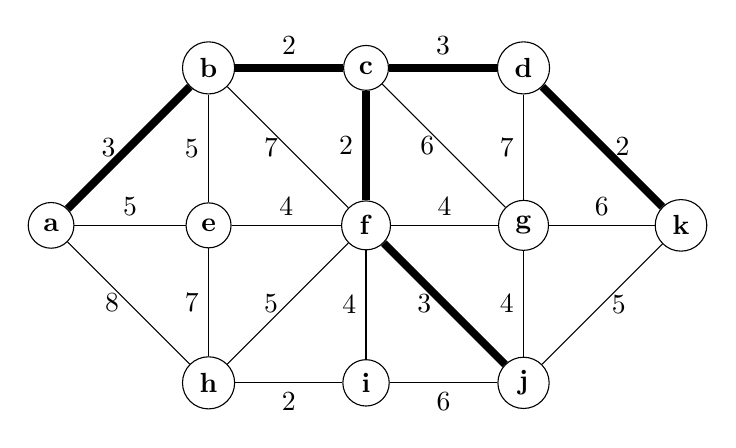
\begin{tikzpicture}
	\node[shape=circle,draw=black] (a) at (0, 2)     {\textbf{a}};
	\node[shape=circle,draw=black] (b) at (2, 4)     {\textbf{b}};
	\node[shape=circle,draw=black] (c) at (4, 4)     {\textbf{c}};
	\node[shape=circle,draw=black] (d) at (6, 4)     {\textbf{d}};
	\node[shape=circle,draw=black] (e) at (2, 2)     {\textbf{e}};
	\node[shape=circle,draw=black] (f) at (4, 2)     {\textbf{f}};
	\node[shape=circle,draw=black] (g) at (6, 2)     {\textbf{g}};
	\node[shape=circle,draw=black] (h) at (2, 0)     {\textbf{h}};
	\node[shape=circle,draw=black] (i) at (4, 0)     {\textbf{i}};
	\node[shape=circle,draw=black] (j) at (6, 0)     {\textbf{j}};
	\node[shape=circle,draw=black] (k) at (8, 2)     {\textbf{k}};
	
	\path[-, line width=1mm] (a) edge node[left]{3} (b);
	\path[-] (a) edge node[above]{5} (e);
	\path[-] (a) edge node[left]{8} (h);
	\path[-] (b) edge node[left]{5} (e);
	\path[-] (b) edge node[left]{7} (f);
	\path[-, line width=1mm] (b) edge node[above]{2} (c);
	\path[-] (e) edge node[above]{4} (f);
	\path[-] (e) edge node[left]{7} (h);
	\path[-] (h) edge node[left]{5} (f);	
	\path[-] (h) edge node[below]{2} (i);	
	\path[- , line width=1mm] (c) edge node[above]{3} (d);
	\path[-] (c) edge node[left]{6} (g);
	\path[-, line width=1mm] (c) edge node[left]{2} (f);
	\path[-] (f) edge node[above]{4} (g);
	\path[-, line width=1mm] (f) edge node[left]{3} (j);
	\path[-] (f) edge node[left]{4} (i);
	\path[-] (i) edge node[below]{6} (j);	
	\path[-, line width=1mm] (d) edge node[right]{2} (k);
	\path[-] (d) edge node[left]{7} (g);
	\path[-] (g) edge node[above]{6} (k);
	\path[-] (g) edge node[left]{4} (j);
	\path[-] (j) edge node[right]{5} (k);
	\end{tikzpicture} 
	\\
	If we control each incident edges to the current vertices our spanning tree has, we can easily see that ${f,j}$ has the lowest weight which is 3. Since ${f,j}$ doesn't create any simple circuits on the spanning tree according to the Prim's Algorithm we should add ${f,j}$ to the spanning tree.
	
\end{figure}

\begin{figure}[H]
	\centering
	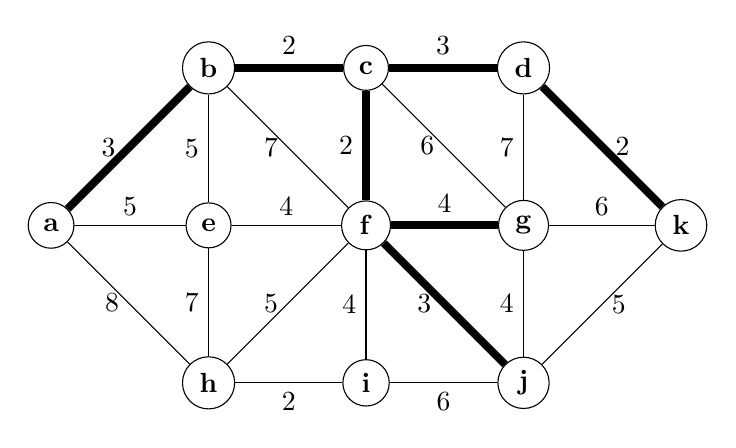
\begin{tikzpicture}
	\node[shape=circle,draw=black] (a) at (0, 2)     {\textbf{a}};
	\node[shape=circle,draw=black] (b) at (2, 4)     {\textbf{b}};
	\node[shape=circle,draw=black] (c) at (4, 4)     {\textbf{c}};
	\node[shape=circle,draw=black] (d) at (6, 4)     {\textbf{d}};
	\node[shape=circle,draw=black] (e) at (2, 2)     {\textbf{e}};
	\node[shape=circle,draw=black] (f) at (4, 2)     {\textbf{f}};
	\node[shape=circle,draw=black] (g) at (6, 2)     {\textbf{g}};
	\node[shape=circle,draw=black] (h) at (2, 0)     {\textbf{h}};
	\node[shape=circle,draw=black] (i) at (4, 0)     {\textbf{i}};
	\node[shape=circle,draw=black] (j) at (6, 0)     {\textbf{j}};
	\node[shape=circle,draw=black] (k) at (8, 2)     {\textbf{k}};
	
	\path[-, line width=1mm] (a) edge node[left]{3} (b);
	\path[-] (a) edge node[above]{5} (e);
	\path[-] (a) edge node[left]{8} (h);
	\path[-] (b) edge node[left]{5} (e);
	\path[-] (b) edge node[left]{7} (f);
	\path[-, line width=1mm] (b) edge node[above]{2} (c);
	\path[-] (e) edge node[above]{4} (f);
	\path[-] (e) edge node[left]{7} (h);
	\path[-] (h) edge node[left]{5} (f);	
	\path[-] (h) edge node[below]{2} (i);	
	\path[- , line width=1mm] (c) edge node[above]{3} (d);
	\path[-] (c) edge node[left]{6} (g);
	\path[-, line width=1mm] (c) edge node[left]{2} (f);
	\path[-, line width=1mm] (f) edge node[above]{4} (g);
	\path[-, line width=1mm] (f) edge node[left]{3} (j);
	\path[-] (f) edge node[left]{4} (i);
	\path[-] (i) edge node[below]{6} (j);	
	\path[-, line width=1mm] (d) edge node[right]{2} (k);
	\path[-] (d) edge node[left]{7} (g);
	\path[-] (g) edge node[above]{6} (k);
	\path[-] (g) edge node[left]{4} (j);
	\path[-] (j) edge node[right]{5} (k);
	\end{tikzpicture} 
	\\
	If we control each incident edges to the current vertices our spanning tree has, we can easily see that ${f,g}$, ${f,i}$, ${f,e}$ have the lowest weight which is 4. Since each of those edges doesn't create any simple circuits on the spanning tree according to the Prim's Algorithm we can add any of them to the spanning tree. At this point, I choose ${f,g}$ to add our spanning tree.
	
\end{figure}

\begin{figure}[H]
	\centering
	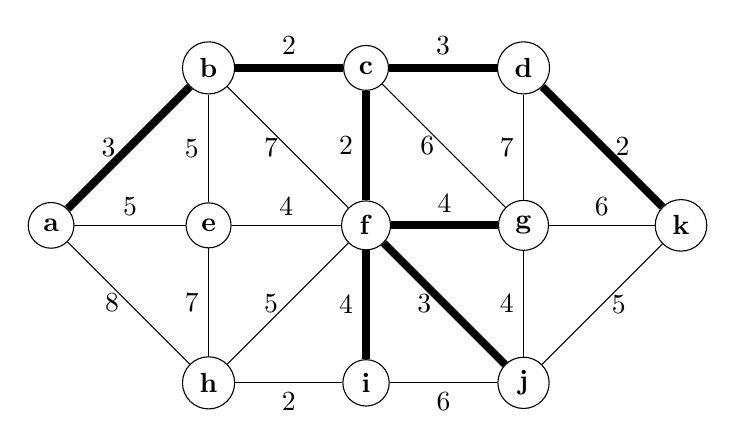
\begin{tikzpicture}
	\node[shape=circle,draw=black] (a) at (0, 2)     {\textbf{a}};
	\node[shape=circle,draw=black] (b) at (2, 4)     {\textbf{b}};
	\node[shape=circle,draw=black] (c) at (4, 4)     {\textbf{c}};
	\node[shape=circle,draw=black] (d) at (6, 4)     {\textbf{d}};
	\node[shape=circle,draw=black] (e) at (2, 2)     {\textbf{e}};
	\node[shape=circle,draw=black] (f) at (4, 2)     {\textbf{f}};
	\node[shape=circle,draw=black] (g) at (6, 2)     {\textbf{g}};
	\node[shape=circle,draw=black] (h) at (2, 0)     {\textbf{h}};
	\node[shape=circle,draw=black] (i) at (4, 0)     {\textbf{i}};
	\node[shape=circle,draw=black] (j) at (6, 0)     {\textbf{j}};
	\node[shape=circle,draw=black] (k) at (8, 2)     {\textbf{k}};
	
	\path[-, line width=1mm] (a) edge node[left]{3} (b);
	\path[-] (a) edge node[above]{5} (e);
	\path[-] (a) edge node[left]{8} (h);
	\path[-] (b) edge node[left]{5} (e);
	\path[-] (b) edge node[left]{7} (f);
	\path[-, line width=1mm] (b) edge node[above]{2} (c);
	\path[-] (e) edge node[above]{4} (f);
	\path[-] (e) edge node[left]{7} (h);
	\path[-] (h) edge node[left]{5} (f);	
	\path[-] (h) edge node[below]{2} (i);	
	\path[- , line width=1mm] (c) edge node[above]{3} (d);
	\path[-] (c) edge node[left]{6} (g);
	\path[-, line width=1mm] (c) edge node[left]{2} (f);
	\path[-, line width=1mm] (f) edge node[above]{4} (g);
	\path[-, line width=1mm] (f) edge node[left]{3} (j);
	\path[-, line width=1mm] (f) edge node[left]{4} (i);
	\path[-] (i) edge node[below]{6} (j);	
	\path[-, line width=1mm] (d) edge node[right]{2} (k);
	\path[-] (d) edge node[left]{7} (g);
	\path[-] (g) edge node[above]{6} (k);
	\path[-] (g) edge node[left]{4} (j);
	\path[-] (j) edge node[right]{5} (k);
	\end{tikzpicture} 
	\\
	If we control each incident edges to the current vertices our spanning tree has, we can easily see that ${g,j}$, ${f,i}$, ${f,e}$ have the lowest weight which is 4. However, we can't add ${g,j}$ to the spanning tree since it creates simple circuit on the spanning tree. Both ${f,i}$ and ${f,e}$ doesn't cause simple circuit on the spanning tree. At this point, I choose ${f,i}$ to add the spanning tree.
	
\end{figure}
\begin{figure}[H]
	\centering
	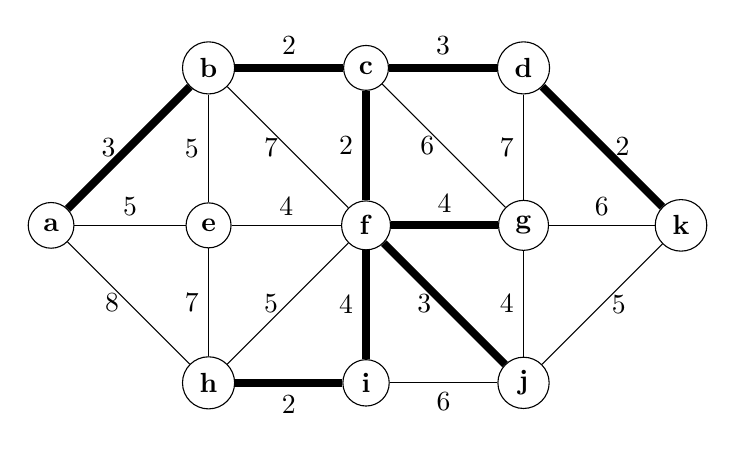
\begin{tikzpicture}
	\node[shape=circle,draw=black] (a) at (0, 2)     {\textbf{a}};
	\node[shape=circle,draw=black] (b) at (2, 4)     {\textbf{b}};
	\node[shape=circle,draw=black] (c) at (4, 4)     {\textbf{c}};
	\node[shape=circle,draw=black] (d) at (6, 4)     {\textbf{d}};
	\node[shape=circle,draw=black] (e) at (2, 2)     {\textbf{e}};
	\node[shape=circle,draw=black] (f) at (4, 2)     {\textbf{f}};
	\node[shape=circle,draw=black] (g) at (6, 2)     {\textbf{g}};
	\node[shape=circle,draw=black] (h) at (2, 0)     {\textbf{h}};
	\node[shape=circle,draw=black] (i) at (4, 0)     {\textbf{i}};
	\node[shape=circle,draw=black] (j) at (6, 0)     {\textbf{j}};
	\node[shape=circle,draw=black] (k) at (8, 2)     {\textbf{k}};
	
	\path[-, line width=1mm] (a) edge node[left]{3} (b);
	\path[-] (a) edge node[above]{5} (e);
	\path[-] (a) edge node[left]{8} (h);
	\path[-] (b) edge node[left]{5} (e);
	\path[-] (b) edge node[left]{7} (f);
	\path[-, line width=1mm] (b) edge node[above]{2} (c);
	\path[-] (e) edge node[above]{4} (f);
	\path[-] (e) edge node[left]{7} (h);
	\path[-] (h) edge node[left]{5} (f);	
	\path[-, line width=1mm] (h) edge node[below]{2} (i);	
	\path[- , line width=1mm] (c) edge node[above]{3} (d);
	\path[-] (c) edge node[left]{6} (g);
	\path[-, line width=1mm] (c) edge node[left]{2} (f);
	\path[-, line width=1mm] (f) edge node[above]{4} (g);
	\path[-, line width=1mm] (f) edge node[left]{3} (j);
	\path[-, line width=1mm] (f) edge node[left]{4} (i);
	\path[-] (i) edge node[below]{6} (j);	
	\path[-, line width=1mm] (d) edge node[right]{2} (k);
	\path[-] (d) edge node[left]{7} (g);
	\path[-] (g) edge node[above]{6} (k);
	\path[-] (g) edge node[left]{4} (j);
	\path[-] (j) edge node[right]{5} (k);
	\end{tikzpicture} 
	\\
	If we control each incident edges to the current vertices our spanning tree has, we can easily see that ${i,h}$ has the lowest weight which is 2. Since ${i,h}$ doesn't create any simple circuit on the spanning tree, we should add it to the spanning tree.
	
\end{figure}

\begin{figure}[H]
	\centering
	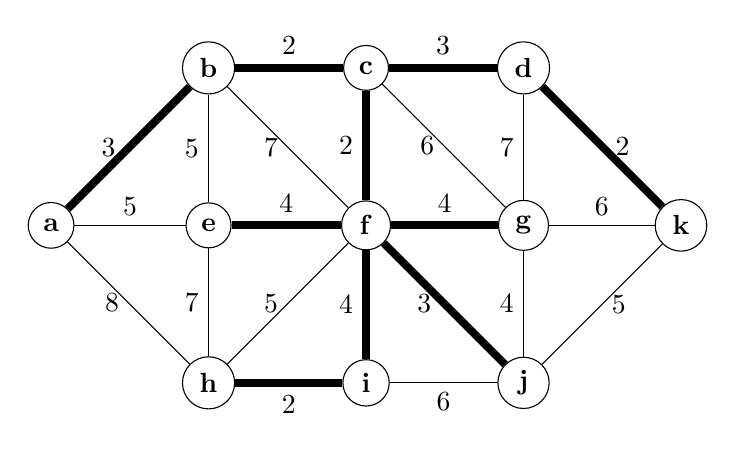
\begin{tikzpicture}
	\node[shape=circle,draw=black] (a) at (0, 2)     {\textbf{a}};
	\node[shape=circle,draw=black] (b) at (2, 4)     {\textbf{b}};
	\node[shape=circle,draw=black] (c) at (4, 4)     {\textbf{c}};
	\node[shape=circle,draw=black] (d) at (6, 4)     {\textbf{d}};
	\node[shape=circle,draw=black] (e) at (2, 2)     {\textbf{e}};
	\node[shape=circle,draw=black] (f) at (4, 2)     {\textbf{f}};
	\node[shape=circle,draw=black] (g) at (6, 2)     {\textbf{g}};
	\node[shape=circle,draw=black] (h) at (2, 0)     {\textbf{h}};
	\node[shape=circle,draw=black] (i) at (4, 0)     {\textbf{i}};
	\node[shape=circle,draw=black] (j) at (6, 0)     {\textbf{j}};
	\node[shape=circle,draw=black] (k) at (8, 2)     {\textbf{k}};
	
	\path[-, line width=1mm] (a) edge node[left]{3} (b);
	\path[-] (a) edge node[above]{5} (e);
	\path[-] (a) edge node[left]{8} (h);
	\path[-] (b) edge node[left]{5} (e);
	\path[-] (b) edge node[left]{7} (f);
	\path[-, line width=1mm] (b) edge node[above]{2} (c);
	\path[-, line width=1mm] (e) edge node[above]{4} (f);
	\path[-] (e) edge node[left]{7} (h);
	\path[-] (h) edge node[left]{5} (f);	
	\path[-, line width=1mm] (h) edge node[below]{2} (i);	
	\path[- , line width=1mm] (c) edge node[above]{3} (d);
	\path[-] (c) edge node[left]{6} (g);
	\path[-, line width=1mm] (c) edge node[left]{2} (f);
	\path[-, line width=1mm] (f) edge node[above]{4} (g);
	\path[-, line width=1mm] (f) edge node[left]{3} (j);
	\path[-, line width=1mm] (f) edge node[left]{4} (i);
	\path[-] (i) edge node[below]{6} (j);	
	\path[-, line width=1mm] (d) edge node[right]{2} (k);
	\path[-] (d) edge node[left]{7} (g);
	\path[-] (g) edge node[above]{6} (k);
	\path[-] (g) edge node[left]{4} (j);
	\path[-] (j) edge node[right]{5} (k);
	\end{tikzpicture} 
	\\
	At this point, we have visited all the vertices on the graph except $e$.
	If we control each incident edges to the current vertices our spanning tree has, we can easily see that ${g,j}$ and ${f,e}$ has the lowest weight which is 4. However, since ${g,j}$ create simple circuit on the spanning tree, according to Prim's Algorithm we can't add it to the spanning tree. So we should add ${f,e}$ to the spanning tree. \\
	
	\end{figure}
	
	Since we add $vertex \ number-1 = 10$ edges to our spanning tree we should stop, we obtained our spanning tree using Prim's Algorithm; \\
	
	\begin{figure}[H]
		\centering
		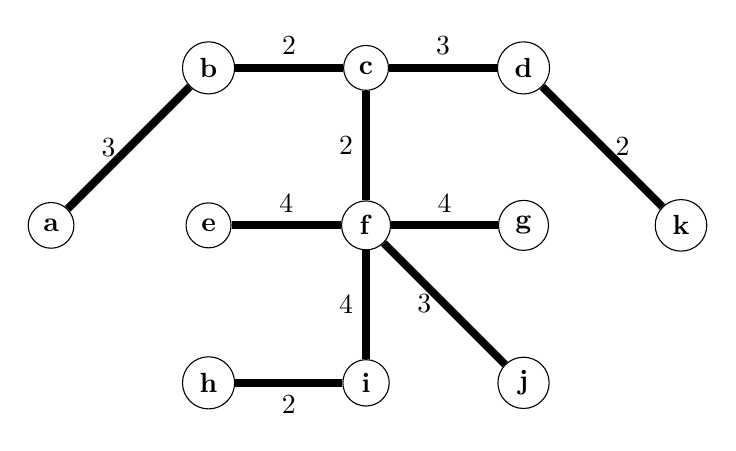
\begin{tikzpicture}
		\node[shape=circle,draw=black] (a) at (0, 2)     {\textbf{a}};
		\node[shape=circle,draw=black] (b) at (2, 4)     {\textbf{b}};
		\node[shape=circle,draw=black] (c) at (4, 4)     {\textbf{c}};
		\node[shape=circle,draw=black] (d) at (6, 4)     {\textbf{d}};
		\node[shape=circle,draw=black] (e) at (2, 2)     {\textbf{e}};
		\node[shape=circle,draw=black] (f) at (4, 2)     {\textbf{f}};
		\node[shape=circle,draw=black] (g) at (6, 2)     {\textbf{g}};
		\node[shape=circle,draw=black] (h) at (2, 0)     {\textbf{h}};
		\node[shape=circle,draw=black] (i) at (4, 0)     {\textbf{i}};
		\node[shape=circle,draw=black] (j) at (6, 0)     {\textbf{j}};
		\node[shape=circle,draw=black] (k) at (8, 2)     {\textbf{k}};
		
		\path[-, line width=1mm] (a) edge node[left]{3} (b);
		\path[-, line width=1mm] (b) edge node[above]{2} (c);
		\path[-, line width=1mm] (e) edge node[above]{4} (f);
		\path[-, line width=1mm] (h) edge node[below]{2} (i);	
		\path[- , line width=1mm] (c) edge node[above]{3} (d);
		\path[-, line width=1mm] (c) edge node[left]{2} (f);
		\path[-, line width=1mm] (f) edge node[above]{4} (g);
		\path[-, line width=1mm] (f) edge node[left]{3} (j);
		\path[-, line width=1mm] (f) edge node[left]{4} (i);
		\path[-, line width=1mm] (d) edge node[right]{2} (k);
		\end{tikzpicture} 
	
\end{figure}

\pagebreak
\section*{Answer 6}
\subsection*{a)}
\textbf{Number of Vertices:} 7 \\
\textbf{Number of Edges:} 6\\
\textbf{Height of the T:} 3
\subsection*{b)}
Preorder: a,b,c,d,e,f,g
\subsection*{c)}
Postorder: b,d,f,g,e,c,a
\subsection*{d)}
Inorder: b,a,d,c,f,e,g
\subsection*{e)}
Since every internal vertex of T which are a,c and e has exactly two children, by the definition T is a full binary tree.
\subsection*{f)}
Since b has no children, level 2 is not completely full. Hence, by the definition, T is not a complete binary tree.
\subsection*{g)}
According to the definition of binary search tree, for an arbitrary binary tree which can be entitled as A, if A is a binary search tree under comparison with respect to $\leq$ relation defined on $Z \times Z$ then for every chosen vertex of A, key of the chosen vertex must not be smaller than the keys of all vertices in its left subtree and must not be bigger than the keys of all vertices in its right subtree. As can be observed, the key of $c$ vertex of $T$ which is 24 is bigger than the key of $f$ which placed in the right subtree of $c$. Hence, T doesn't satisfy the definition of binary search tree under comparison with respect to $\leq$ relation. Thus, T is not a binary search tree.
\subsection*{h)}
Minimum number of nodes for a full binary tree with height 5 can be obtained from the below case; \\
\begin{figure}[H]
	\centering
	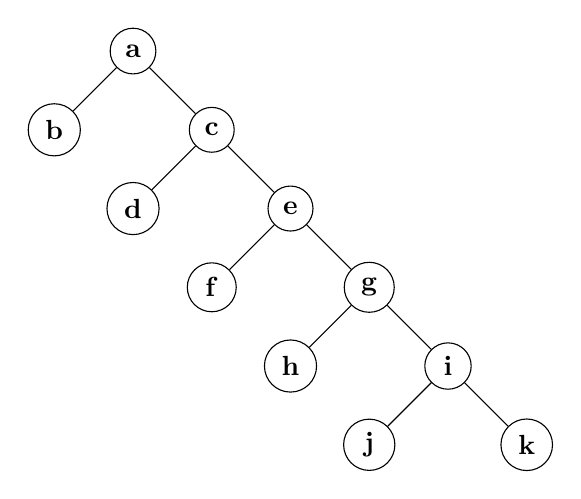
\begin{tikzpicture}
	\node[shape=circle,draw=black] (a) at (1, 8)     {\textbf{a}};
	\node[shape=circle,draw=black] (b) at (0, 7)     {\textbf{b}};
	\node[shape=circle,draw=black] (c) at (2, 7)     {\textbf{c}};
	\node[shape=circle,draw=black] (e) at (3, 6)     {\textbf{e}};
	\node[shape=circle,draw=black] (d) at (1, 6)     {\textbf{d}};
	\node[shape=circle,draw=black] (g) at (4, 5)     {\textbf{g}};
	\node[shape=circle,draw=black] (f) at (2, 5)     {\textbf{f}};
	\node[shape=circle,draw=black] (i) at (5, 4)     {\textbf{i}};
	\node[shape=circle,draw=black] (h) at (3, 4)     {\textbf{h}};
	\node[shape=circle,draw=black] (k) at (6, 3)     {\textbf{k}};
	\node[shape=circle,draw=black] (j) at (4, 3)     {\textbf{j}};
	
	
	\path[-] (a) edge  (b);
	\path[-] (a) edge  (c);
	\path[-] (c) edge  (d);
	\path[-] (c) edge  (e);
	\path[-] (e) edge  (f);
	\path[-] (e) edge  (g);
	\path[-] (g) edge  (h);
	\path[-] (g) edge  (i);
	\path[-] (i) edge  (j);
	\path[-] (i) edge  (k);
	
	
	\end{tikzpicture} 
\end{figure}
As can be seen, given tree is a full binary tree with 5 height and 11 nodes. Thus, minimum number of nodes for a full binary tree with height 5 is 11.

\subsection*{i)}
\begin{figure}[H]
	\centering
	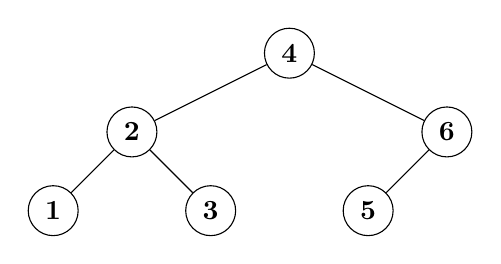
\begin{tikzpicture}
	\node[shape=circle,draw=black] (4) at (3, 2)     {\textbf{4}};
	\node[shape=circle,draw=black] (2) at (1, 1)     {\textbf{2}};
	\node[shape=circle,draw=black] (1) at (0, 0)     {\textbf{1}};
	\node[shape=circle,draw=black] (3) at (2, 0)     {\textbf{3}};
	\node[shape=circle,draw=black] (6) at (5, 1)     {\textbf{6}};
	\node[shape=circle,draw=black] (5) at (4, 0)     {\textbf{5}};

	
	
	
	\path[-] (4) edge  (2);
	\path[-] (4) edge  (6);
	\path[-] (2) edge  (1);
	\path[-] (2) edge  (3);
	\path[-] (6) edge  (5);
	
	
	\end{tikzpicture} 
\end{figure}
\subsection*{j)}
\textbf{For searching 1:} 4,2,1 \\
\textbf{For searching 6:} 4,6 
\subsection*{k)}
\begin{figure}[H]
	\centering
	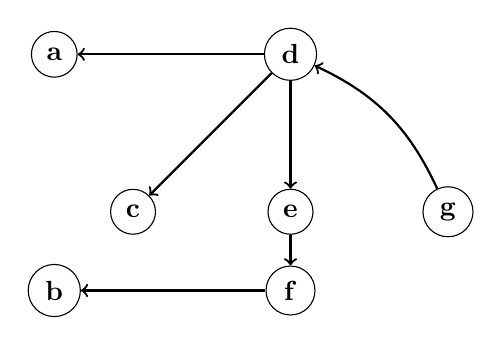
\begin{tikzpicture}
	
	\node[shape=circle,draw=black] (a) at (0, 3)     {\textbf{a}};
	\node[shape=circle,draw=black] (b) at (0, 0)     {\textbf{b}};
	\node[shape=circle,draw=black] (c) at (1, 1)     {\textbf{c}};
	\node[shape=circle,draw=black] (d) at (3, 3)     {\textbf{d}};
	\node[shape=circle,draw=black] (e) at (3, 1)     {\textbf{e}};
	\node[shape=circle,draw=black] (f) at (3, 0)     {\textbf{f}};
	\node[shape=circle,draw=black] (g) at (5, 1)     {\textbf{g}};
	
	\path[->, thick] (g) edge [bend right=20] (d);
	\path[->, thick] (d) edge (e);
	\path[->, thick] (d) edge (c);
	\path[->, thick] (d) edge (a);
	\path[->, thick] (e) edge (f);
	\path[->, thick] (f) edge (b);
	
	\end{tikzpicture} 
\end{figure}
\subsection*{l)}
To obtain the maximum height, binary search tree should be in the linear form.For instance; \\ 
\begin{figure}[H]
	\centering
	\begin{tikzpicture}
	\node[shape=circle,draw=black] (0) at (0, 6)     {\textbf{0}};
	\node[shape=circle,draw=black] (1) at (1, 5)     {\textbf{1}};
	\node[shape=circle,draw=black] (2) at (2, 4)     {\textbf{2}};
	\node[shape=circle,draw=black] (3) at (3, 3)     {\textbf{.}};
	\node[shape=circle,draw=black] (4) at (4, 2)     {\textbf{.}};
	\node[shape=circle,draw=black] (5) at (5, 1)     {\textbf{.}};
	\node[shape=circle,draw=black] (k) at (6, 0)     {\textbf{k-1}};
	
	
	
	
	\path[-] (0) edge  (1);
	\path[-] (1) edge  (2);
	\path[-] (2) edge  (3);
	\path[-] (3) edge  (4);
	\path[-] (4) edge  (5);
	\path[-] (5) edge  (k);
	
	
	\end{tikzpicture} 
\end{figure}
In the described case, height of the tree would be equal to the number of edges which is k-1. Thus, maximum height to create a binary search tree containing k vertices is k-1.
\end{document}

​

